\documentclass{beamer}
\usetheme{Darmstadt}
\usecolortheme{default}

% balíčky

\usepackage[utf8]{inputenc}
\usepackage[czech]{babel}
\usepackage{graphicx}

% informace o dokumentu

\title[Krytosemenné rostliny]{Krytosemenné rostliny}
\subtitle[prezentace do Bi]{prezentace do Bi}
\author{Jiří Kalvoda, Michal Holoubek, Martin Šálek, Vojtěch Blažík, David Procházka}
\date{}

% text dokumentu

\begin{document}

% titulní stránka
% (název prezentace, autor, datum...)

\begin{frame}
  \titlepage
\end{frame}

\begin{frame}
\frametitle{Taxonomické rozdělení}

\begin{center}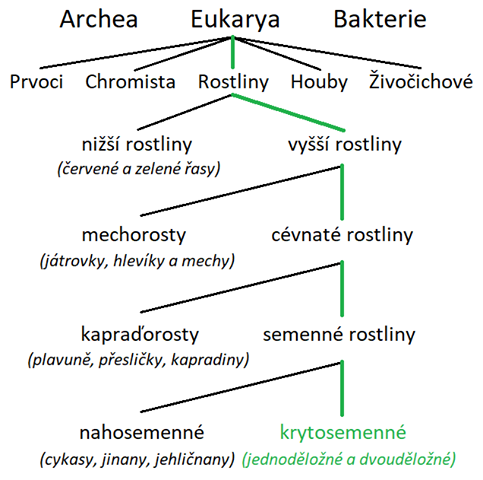
\includegraphics[width=6.5cm]{1.png}\end{center}

\end{frame}
\begin{frame}

\frametitle{Rozdílné znaky}
	\framesubtitle{Počet děloh}

- jednoděložné = jedna děloha

- dvouděložné = dvě dělohy

- existují výjimky (zakrnělé, srostlé)

\end{frame}
\begin{frame}
\frametitle{Rozdílné znaky}
	\framesubtitle{Kořen}

- hlavní a vedlejší (např. u mrkve)

\end{frame}
\begin{frame}
\frametitle{Rozdílné znaky}
	\framesubtitle{Cévní svazky}
- u jednoděložných rozptýlené

- u dvouděložných uspořádané do kruhu (xylém u středu)

- dvouděložné mají kambium, druhotné tloustnutí

\begin{center}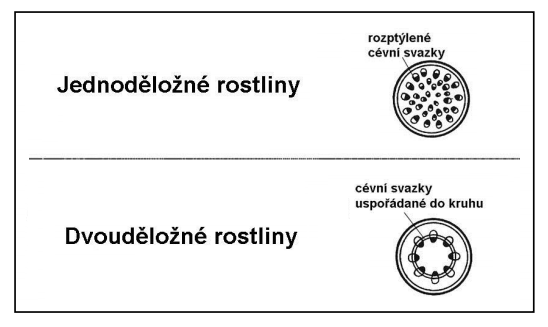
\includegraphics[width=8cm]{3.png}\end{center}

\end{frame}
\begin{frame}
\frametitle{Rozdílné znaky}
	\framesubtitle{Listy}

- u jednoděložných zpravidla jednodušší

- souběžná žilnatina

- většinou ve střídavém uspořádání nebo v růžici

\begin{center}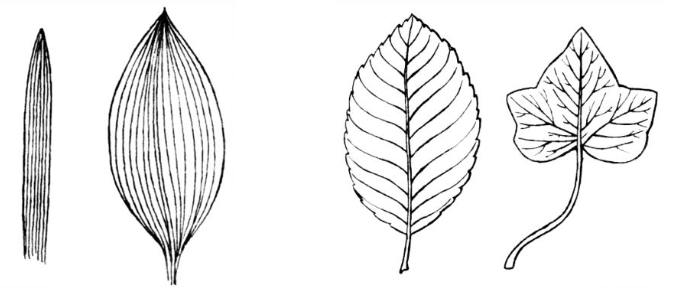
\includegraphics[width=8cm]{2.png}\end{center}

\end{frame}
\begin{frame}
\frametitle{Rozdílné znaky}
	\framesubtitle{Květy}

- okvětí je rozlišené pouze u dvouděložných rostlin (K+K)

- u jednoděložných okvětní lístky po trojicích

- u dvouděložných po čtveřicích až pěticích

\end{frame}
\begin{frame}
\frametitle{Čeledi}
	\framesubtitle{Jednoděložné}

11 řádů, asi 70 čeledí

chřestotvaré (amarylkovité, kosatcovité, vstavačovité),  lipnicotvaré (lipnicovité, šáchorovité), liliotvaré (liliovité)

\begin{center}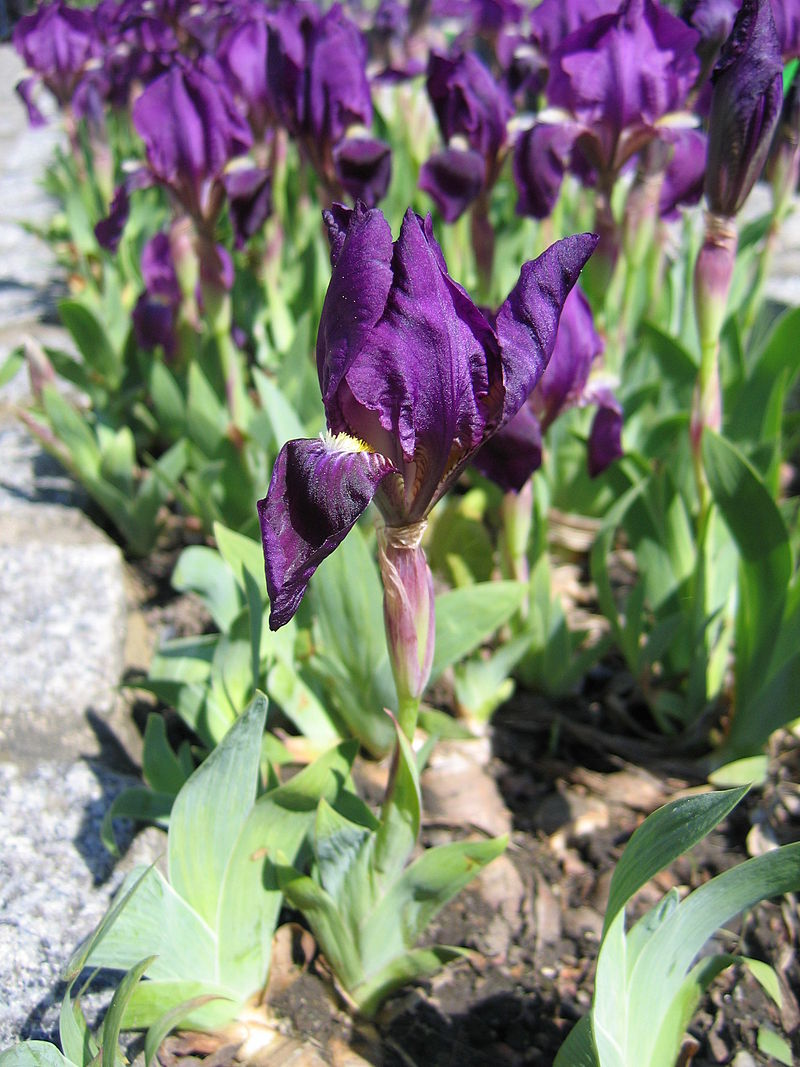
\includegraphics[width=4cm]{800px-Iris_pumila_01.jpg}\end{center}
\end{frame}
\begin{frame}
\frametitle{Čeledi}
	\framesubtitle{Dvouděložné nižší}

9 řádů, asi 30 čeledí

leknínotvaré (leknínovité), šácholanotvaré (šácholanovité)
\begin{center}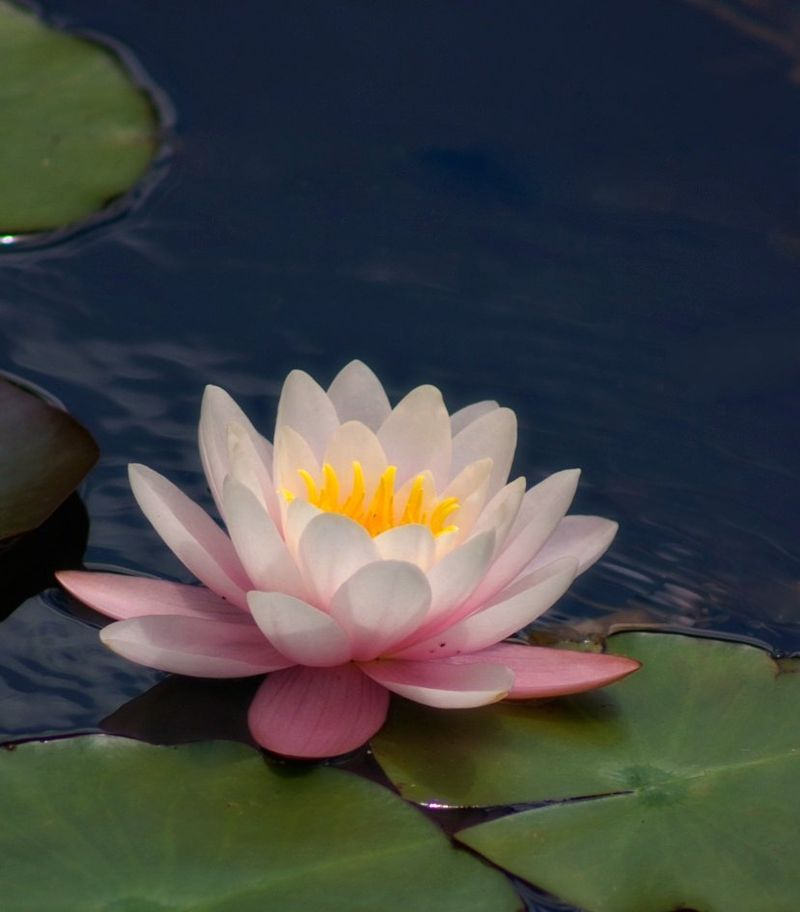
\includegraphics[width=5cm]{30_days_of_gratitude-_Day_1_(4063918440).jpg}\end{center}
\end{frame}
\begin{frame}
\frametitle{Čeledi}
	\framesubtitle{Dvouděložné vyšší}

44 řádů, hodně čeledí

pryskyřníkotvaré (pryskyřníkovité), brukvotvaré (brukvovité), bobotvaré (bobovité), miříkotvaré (miříkovité), hluchavkotvaré (hluchavkovité), hvězdnicovité (hvězdnicotvaré)
\begin{center}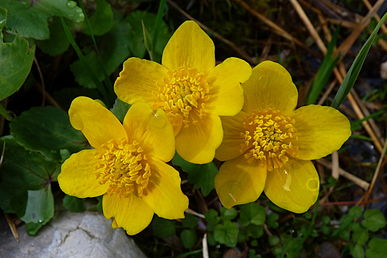
\includegraphics[width=7cm]{387px-Caltha_palustris_a.jpg}\end{center}


\end{frame}
\begin{frame}
\frametitle{Dělení jednoděložných}
\framesubtitle{Amarylkovité}
pozemní byliny, mají cibuli

příklad: narcis žlutý %Narcissus_pseudonarcissus1.jpg

\begin{center}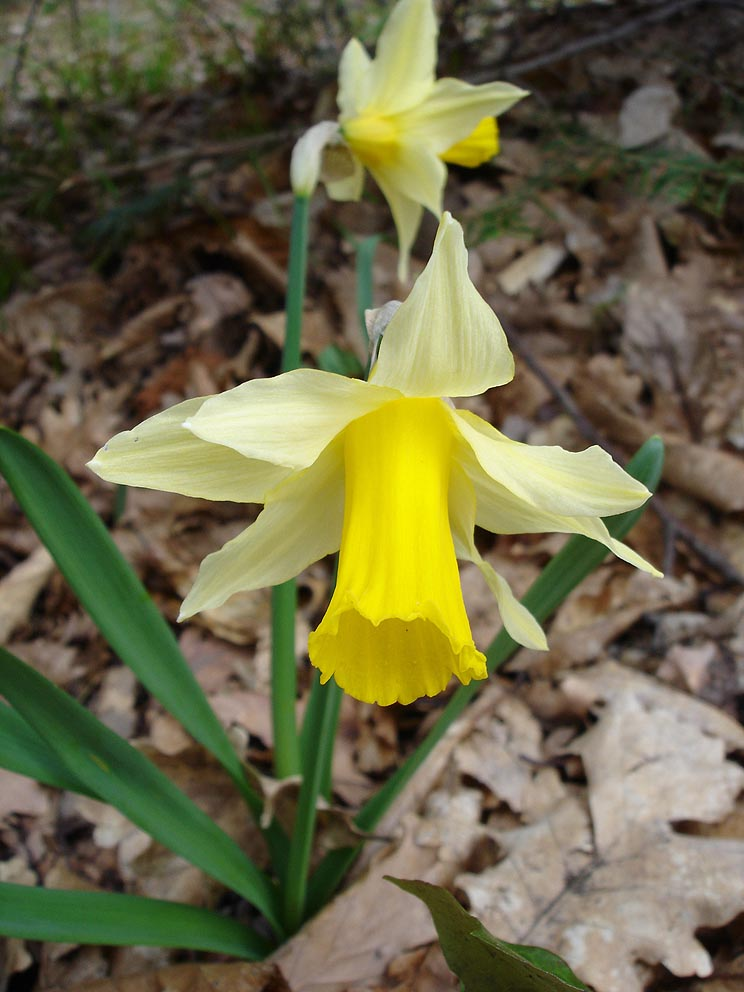
\includegraphics[width=8cm]{Narcissus_pseudonarcissus1.jpg}\end{center}

\end{frame}
\begin{frame}
\frametitle{Dělení jednoděložných}
\framesubtitle{Kosatcovité}

převážně byliny, téměř vždy s oddenkem

příklad: kosatec německý %https://upload.wikimedia.org/wikipedia/commons/9/93/Iris_germanica10.jpg

\begin{center}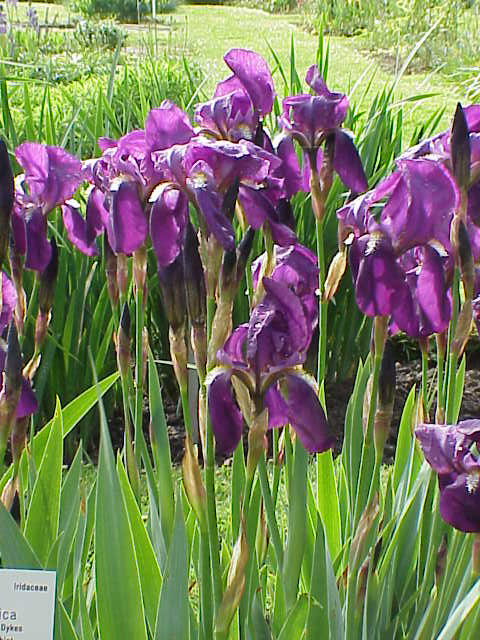
\includegraphics[width=8cm]{Iris_germanica10.jpg}\end{center}

\end{frame}
\begin{frame}
\frametitle{Dělení jednoděložných}
\framesubtitle{Vstavačovité}
vytrvalé byliny

původ v tropických oblastech


příklad: prstnatec májový %https://upload.wikimedia.org/wikipedia/commons/thumb/3/30/Knabenkraut_2286.jpg/800px-Knabenkraut_2286.jpg

\begin{center}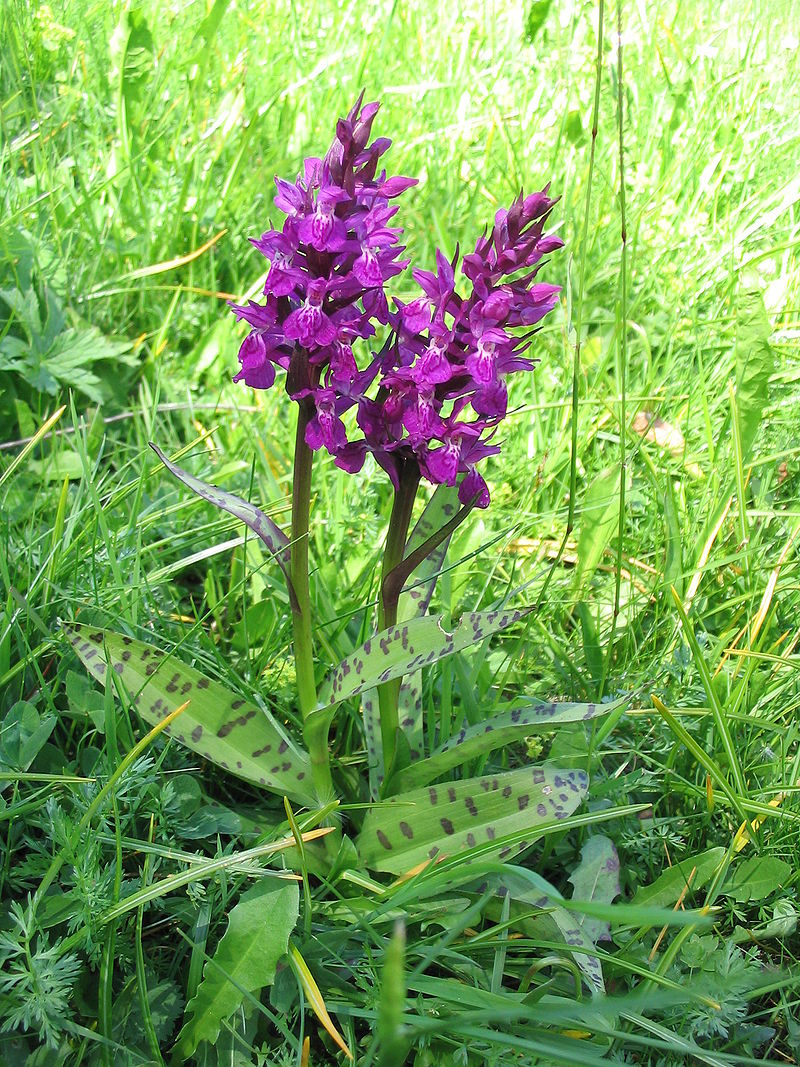
\includegraphics[width=8cm]{800px-Knabenkraut_2286.jpg}\end{center}

\end{frame}
\begin{frame}
\frametitle{Dělení jednoděložných}
\framesubtitle{Lipnicovité}
jinak trávy; byliny nebo dřeviny

příklad: lipnice luční %https://upload.wikimedia.org/wikipedia/commons/thumb/5/5b/Poa_pratensis1.JPG/800px-Poa_pratensis1.JPG

\begin{center}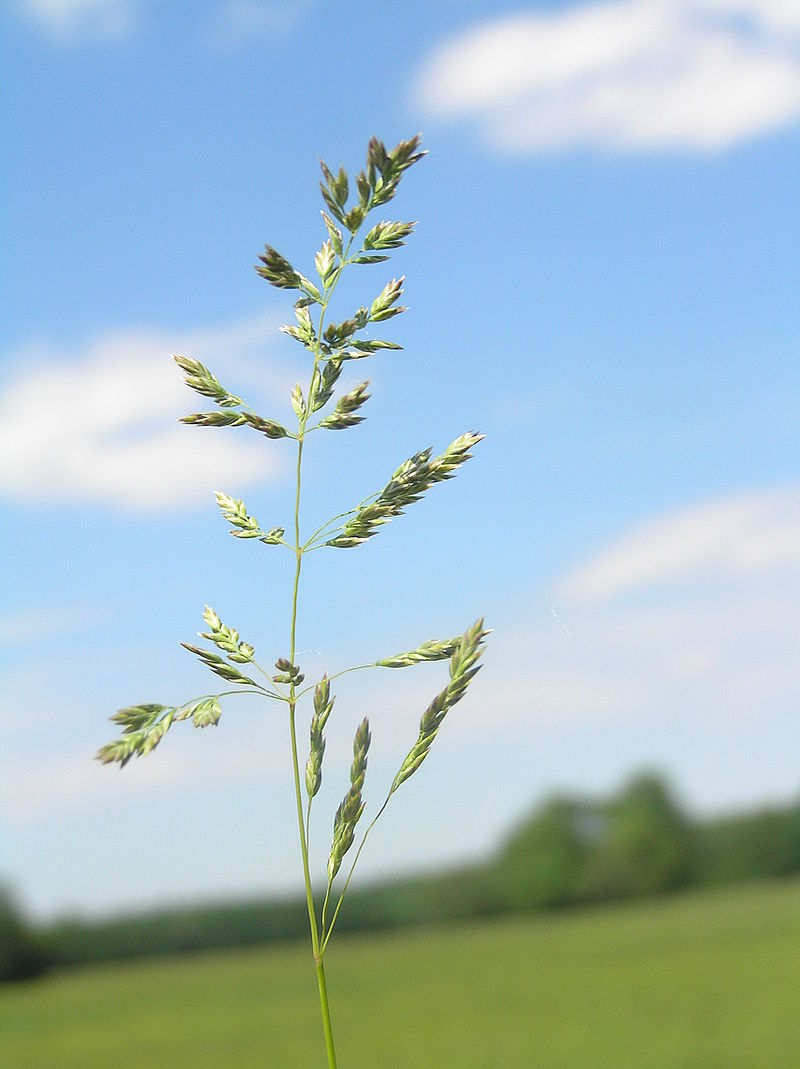
\includegraphics[width=8cm]{800px-Poa_pratensis1.JPG}\end{center}

\end{frame}
\begin{frame}
\frametitle{Dělení jednoděložných}
\framesubtitle{Šáchorovité}
pozemní, nebo vodní byliny (kořeny ve dně)

příklad: skřípina lesní %https://upload.wikimedia.org/wikipedia/commons/thumb/1/11/ScirpusSylvaticus.jpg/800px-ScirpusSylvaticus.jpg

\begin{center}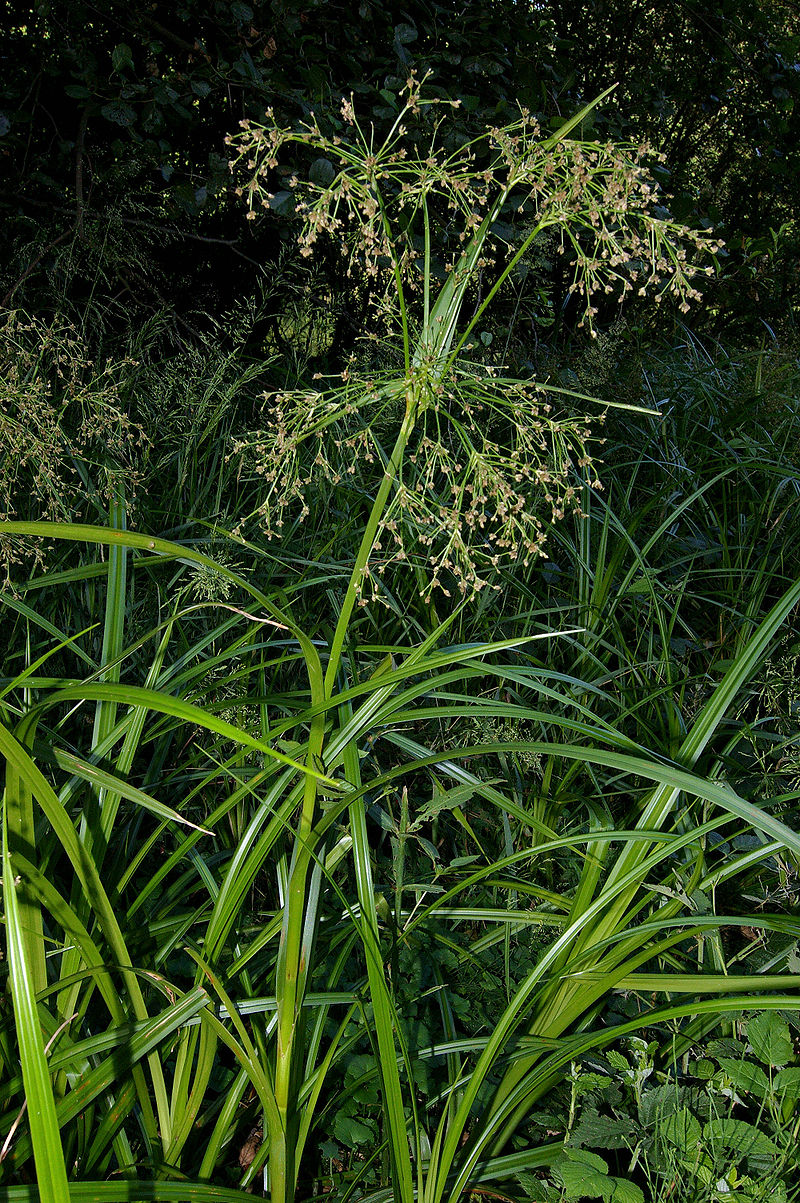
\includegraphics[width=8cm]{800px-ScirpusSylvaticus.jpg}\end{center}

\end{frame}
\begin{frame}
\frametitle{Dělení jednoděložných}
\framesubtitle{Liliovité}
vytrvalé pozemní byliny, mají cibuli

příklad: lilie zlatohlavá

\begin{center}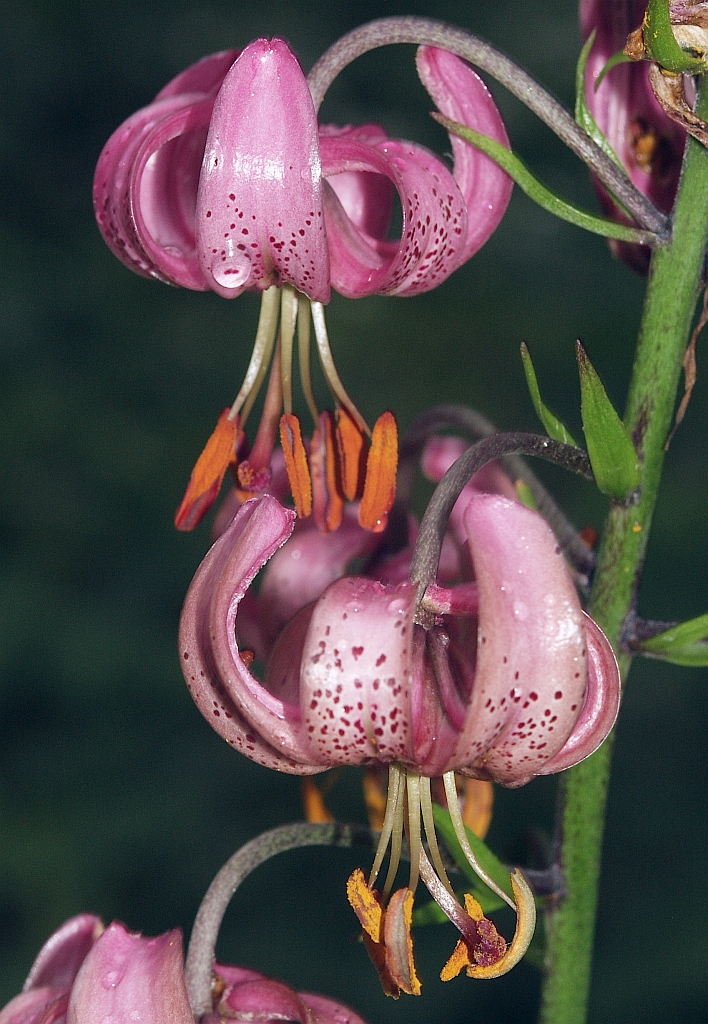
\includegraphics[width=8cm]{Lilium_martagon_250605a.jpg}\end{center}

%tps://upload.wikimedia.org/wikipedia/commons/3/34/Lilium_martagon_250605a.jpg
\end{frame}
\begin{frame}


\frametitle{Dělení dvouděložných}
	\framesubtitle{Šácholánovité}nejstarší

Příklad: magnolie

\begin{center}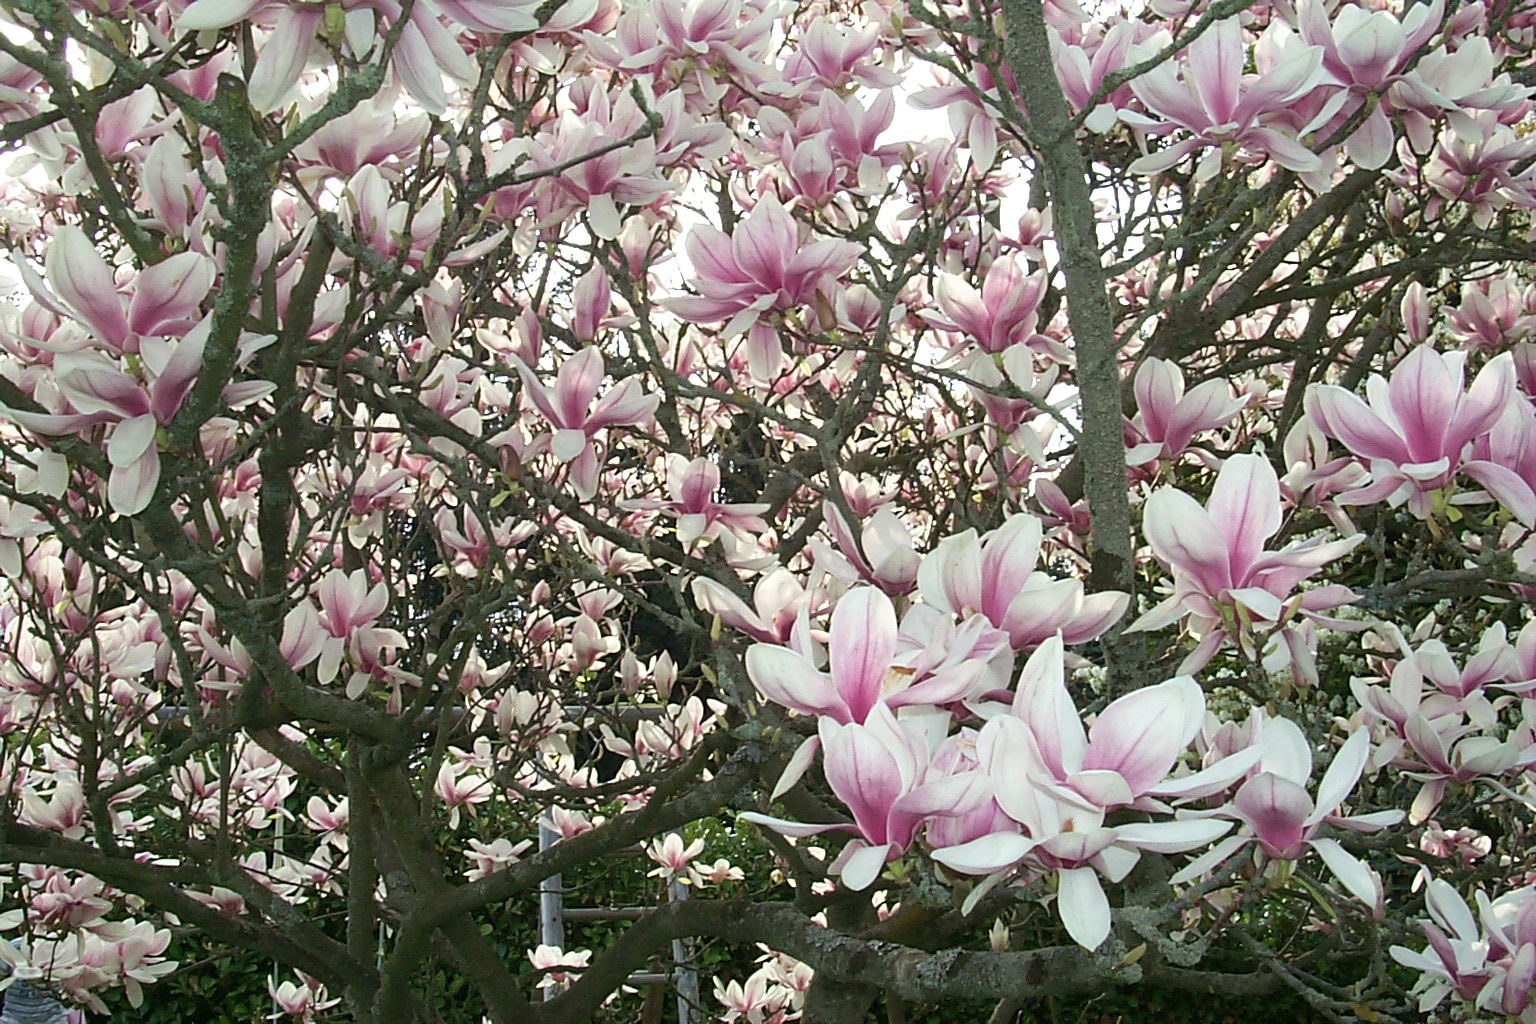
\includegraphics[width=8cm]{Magnolie_in_Wehrheim_-_April_2006.jpg}\end{center}
\end{frame}
\begin{frame}
\frametitle{Dělení dvouděložných}
	\framesubtitle{Leknínovité}Jednoznačně rozeznatelné

Příklad: leknín

\begin{center}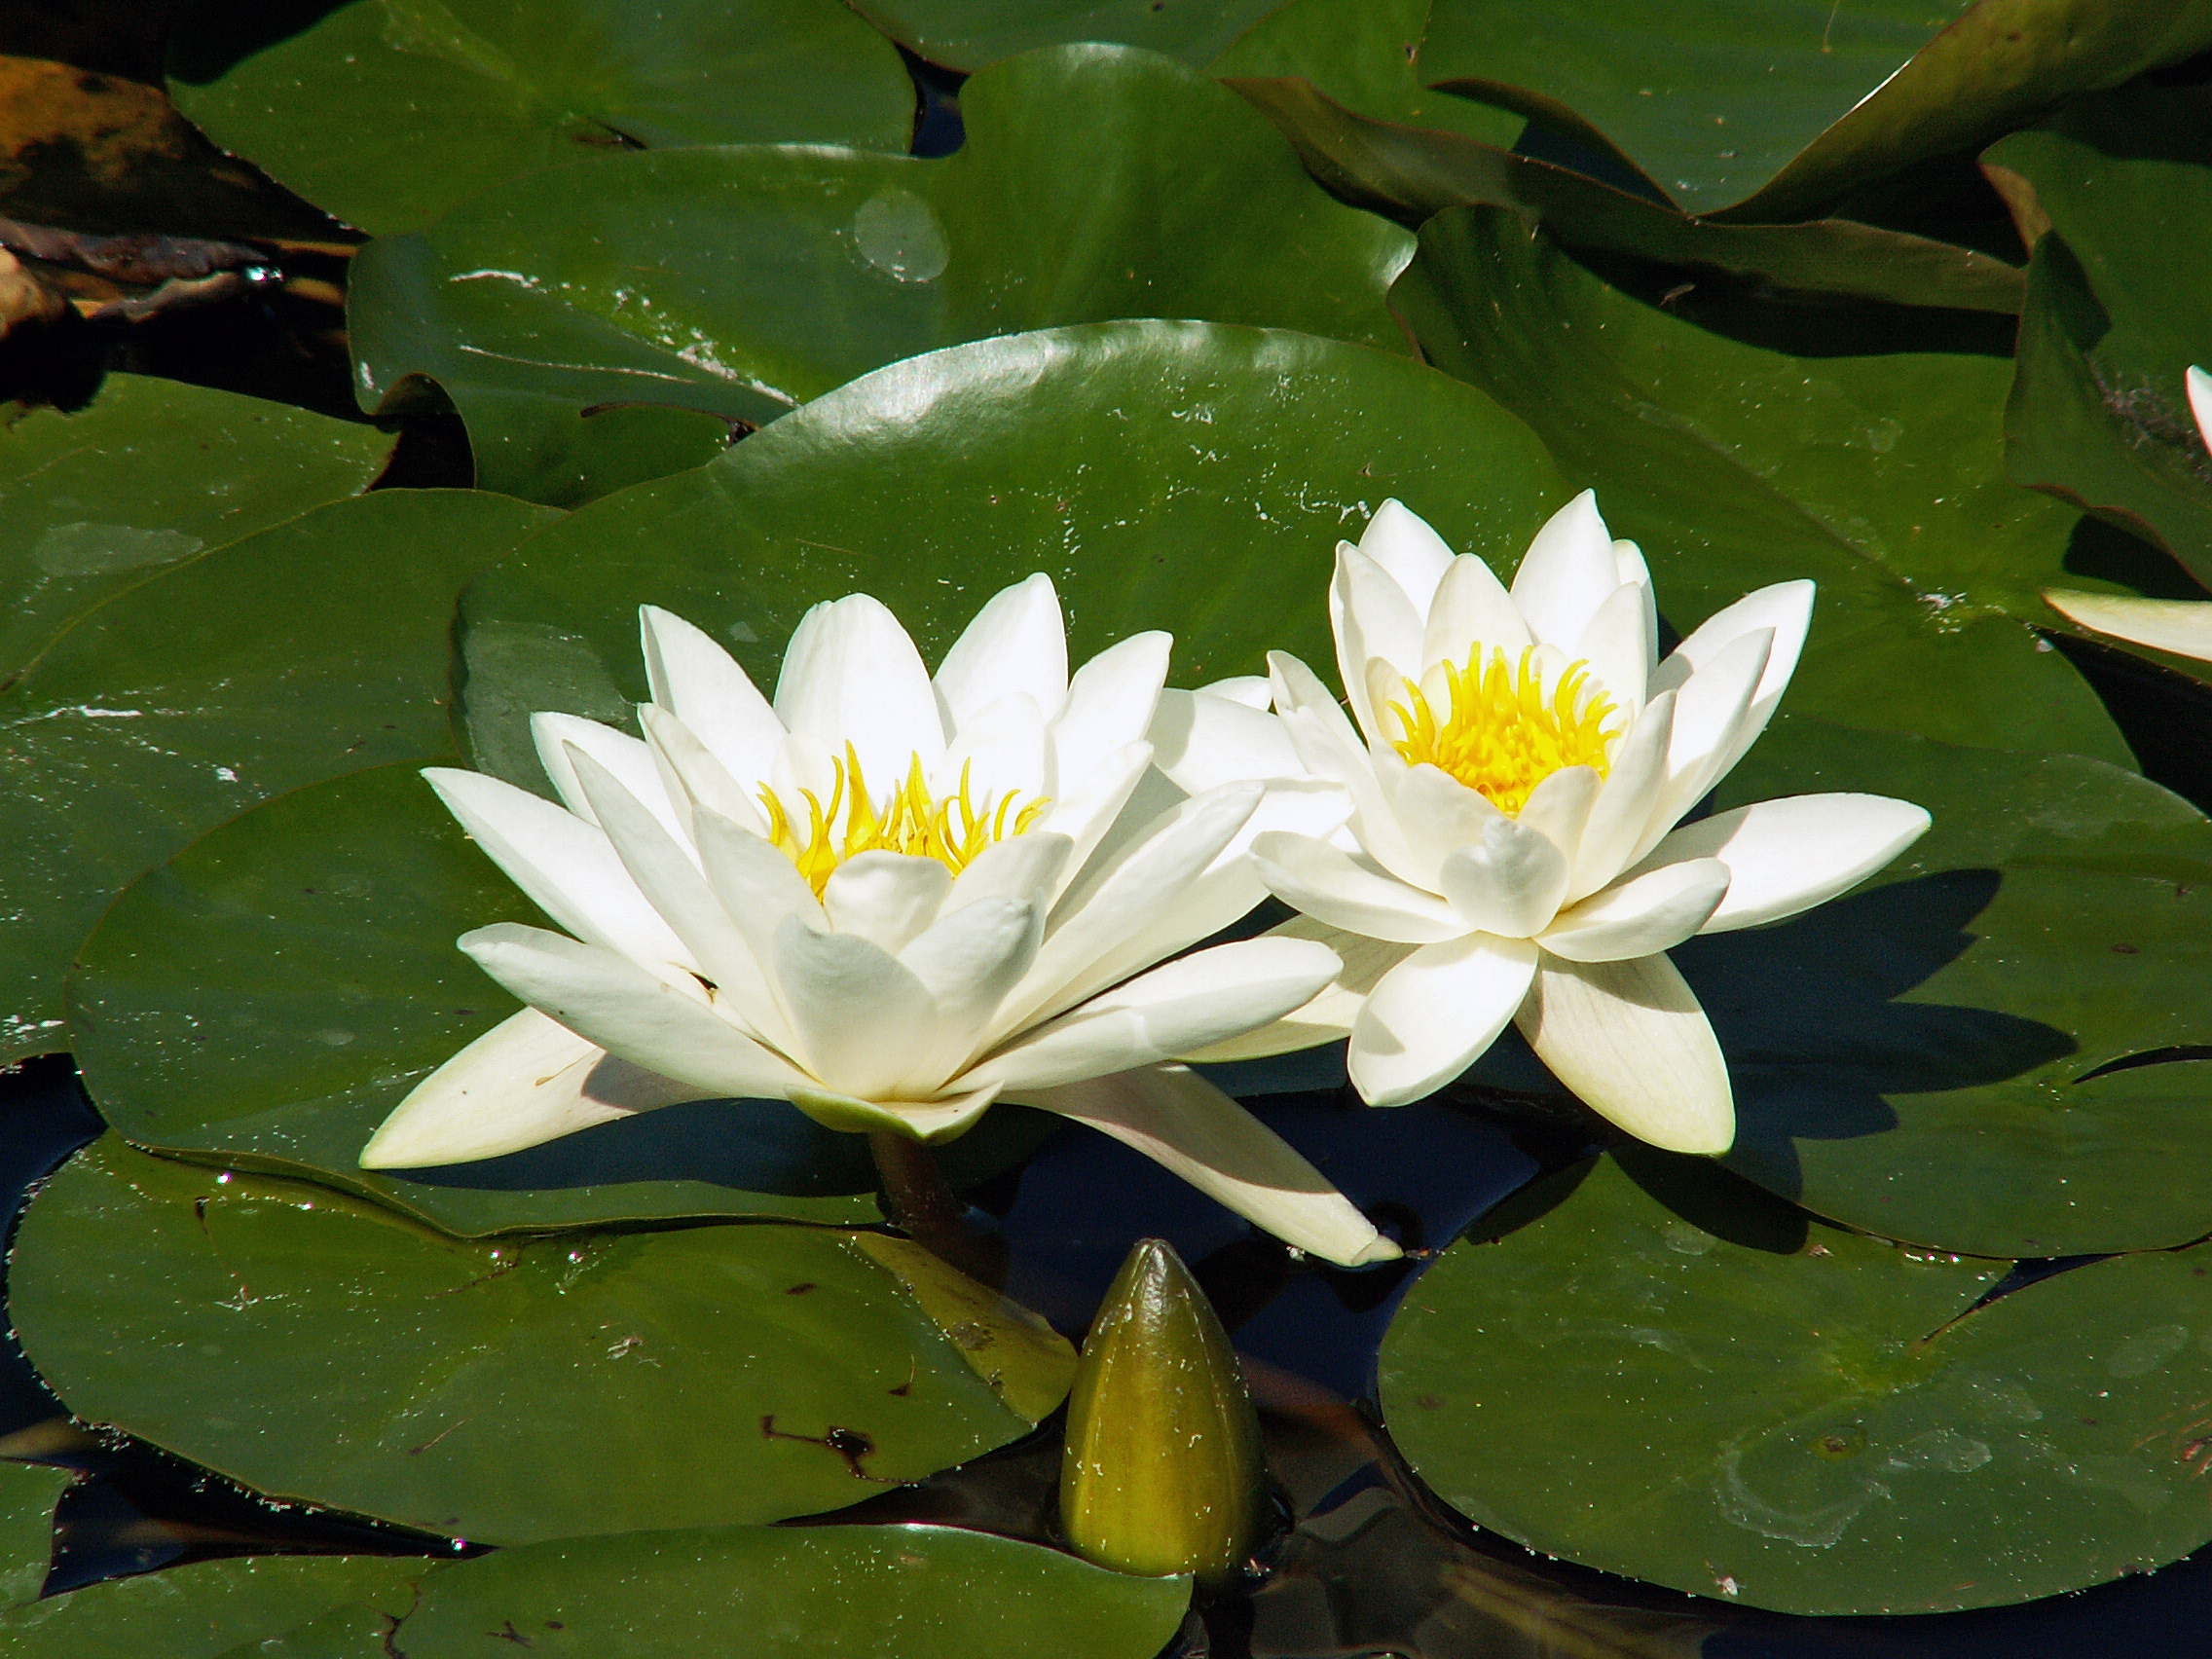
\includegraphics[width=8cm]{Nymphaea_alba_26-8-2007_15-13-19.jpg}\end{center}
\end{frame}
\begin{frame}
\frametitle{Dělení dvouděložných}
	\framesubtitle{Pryskyřníkovité}vytrvalé byliny obsahující alkaloidy

Příklad: pryskyřník prudký

\begin{center}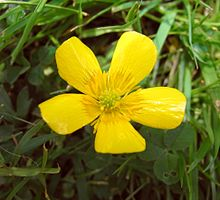
\includegraphics[width=8cm]{220px-A_06_butterblume_2_wp.jpg}\end{center}
\end{frame}
\begin{frame}
\frametitle{Dělení dvouděložných}
	\framesubtitle{Mákovité}alkaloidy v lékařství, obsahují oleje

Příklad: mák setý

\begin{center}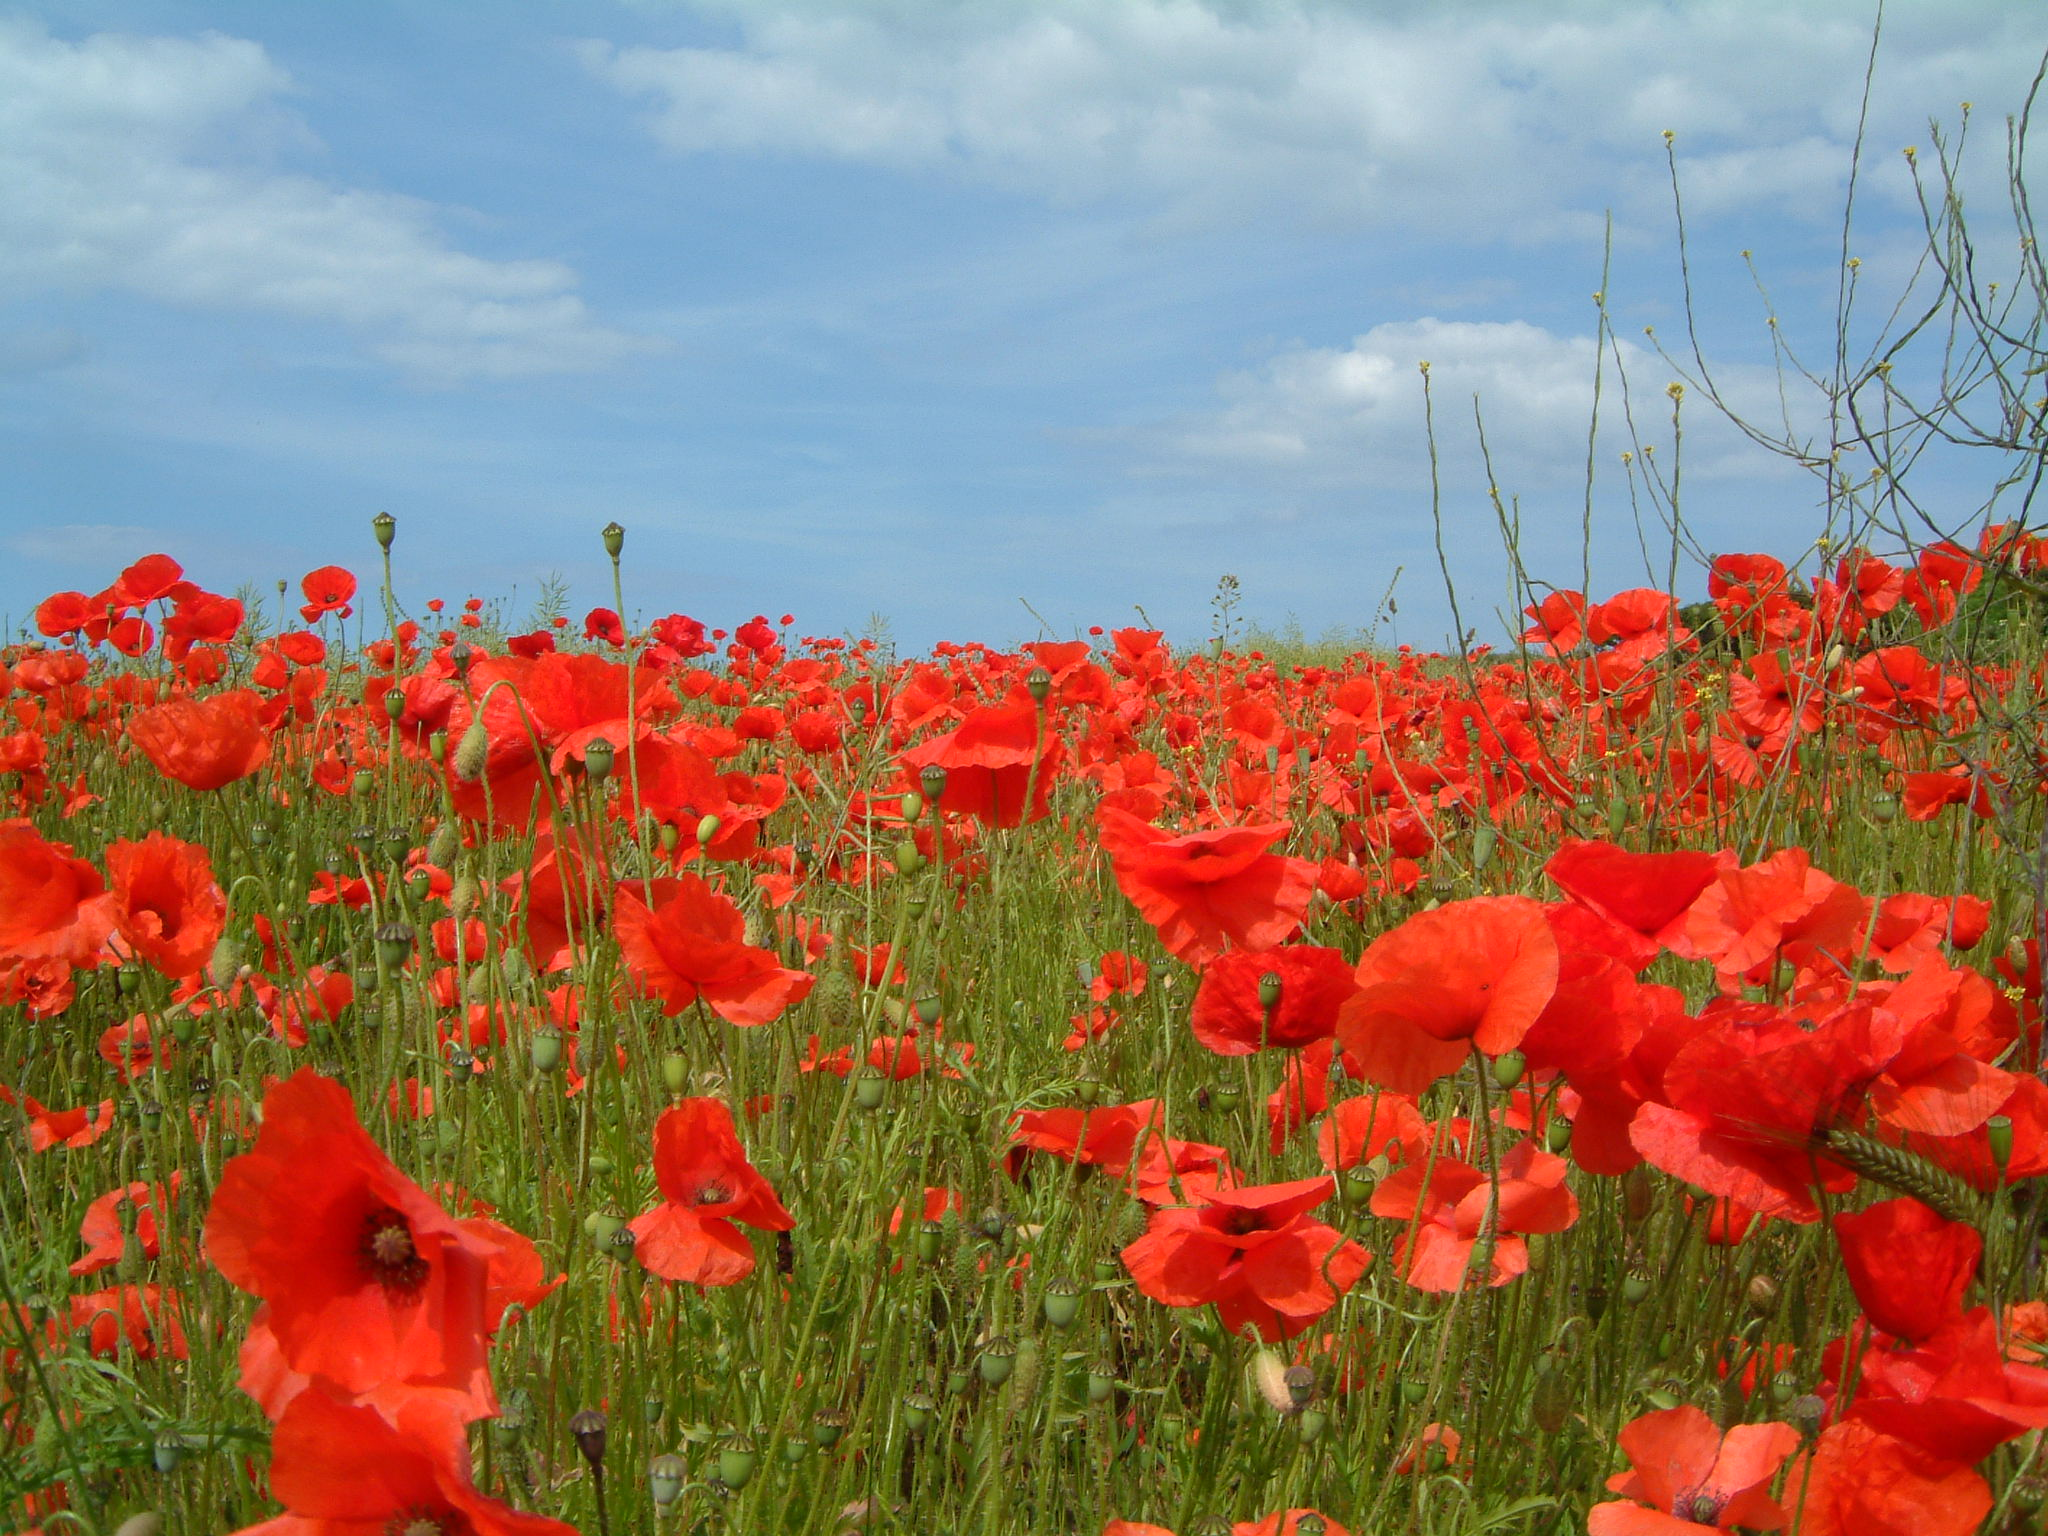
\includegraphics[width=8cm]{Poppy2004.jpg}\end{center}
\end{frame}
\begin{frame}
\frametitle{Dělení dvouděložných}
	\framesubtitle{Morušovníkovité}hlavně dřeviny

Příklad: fíkovník

\begin{center}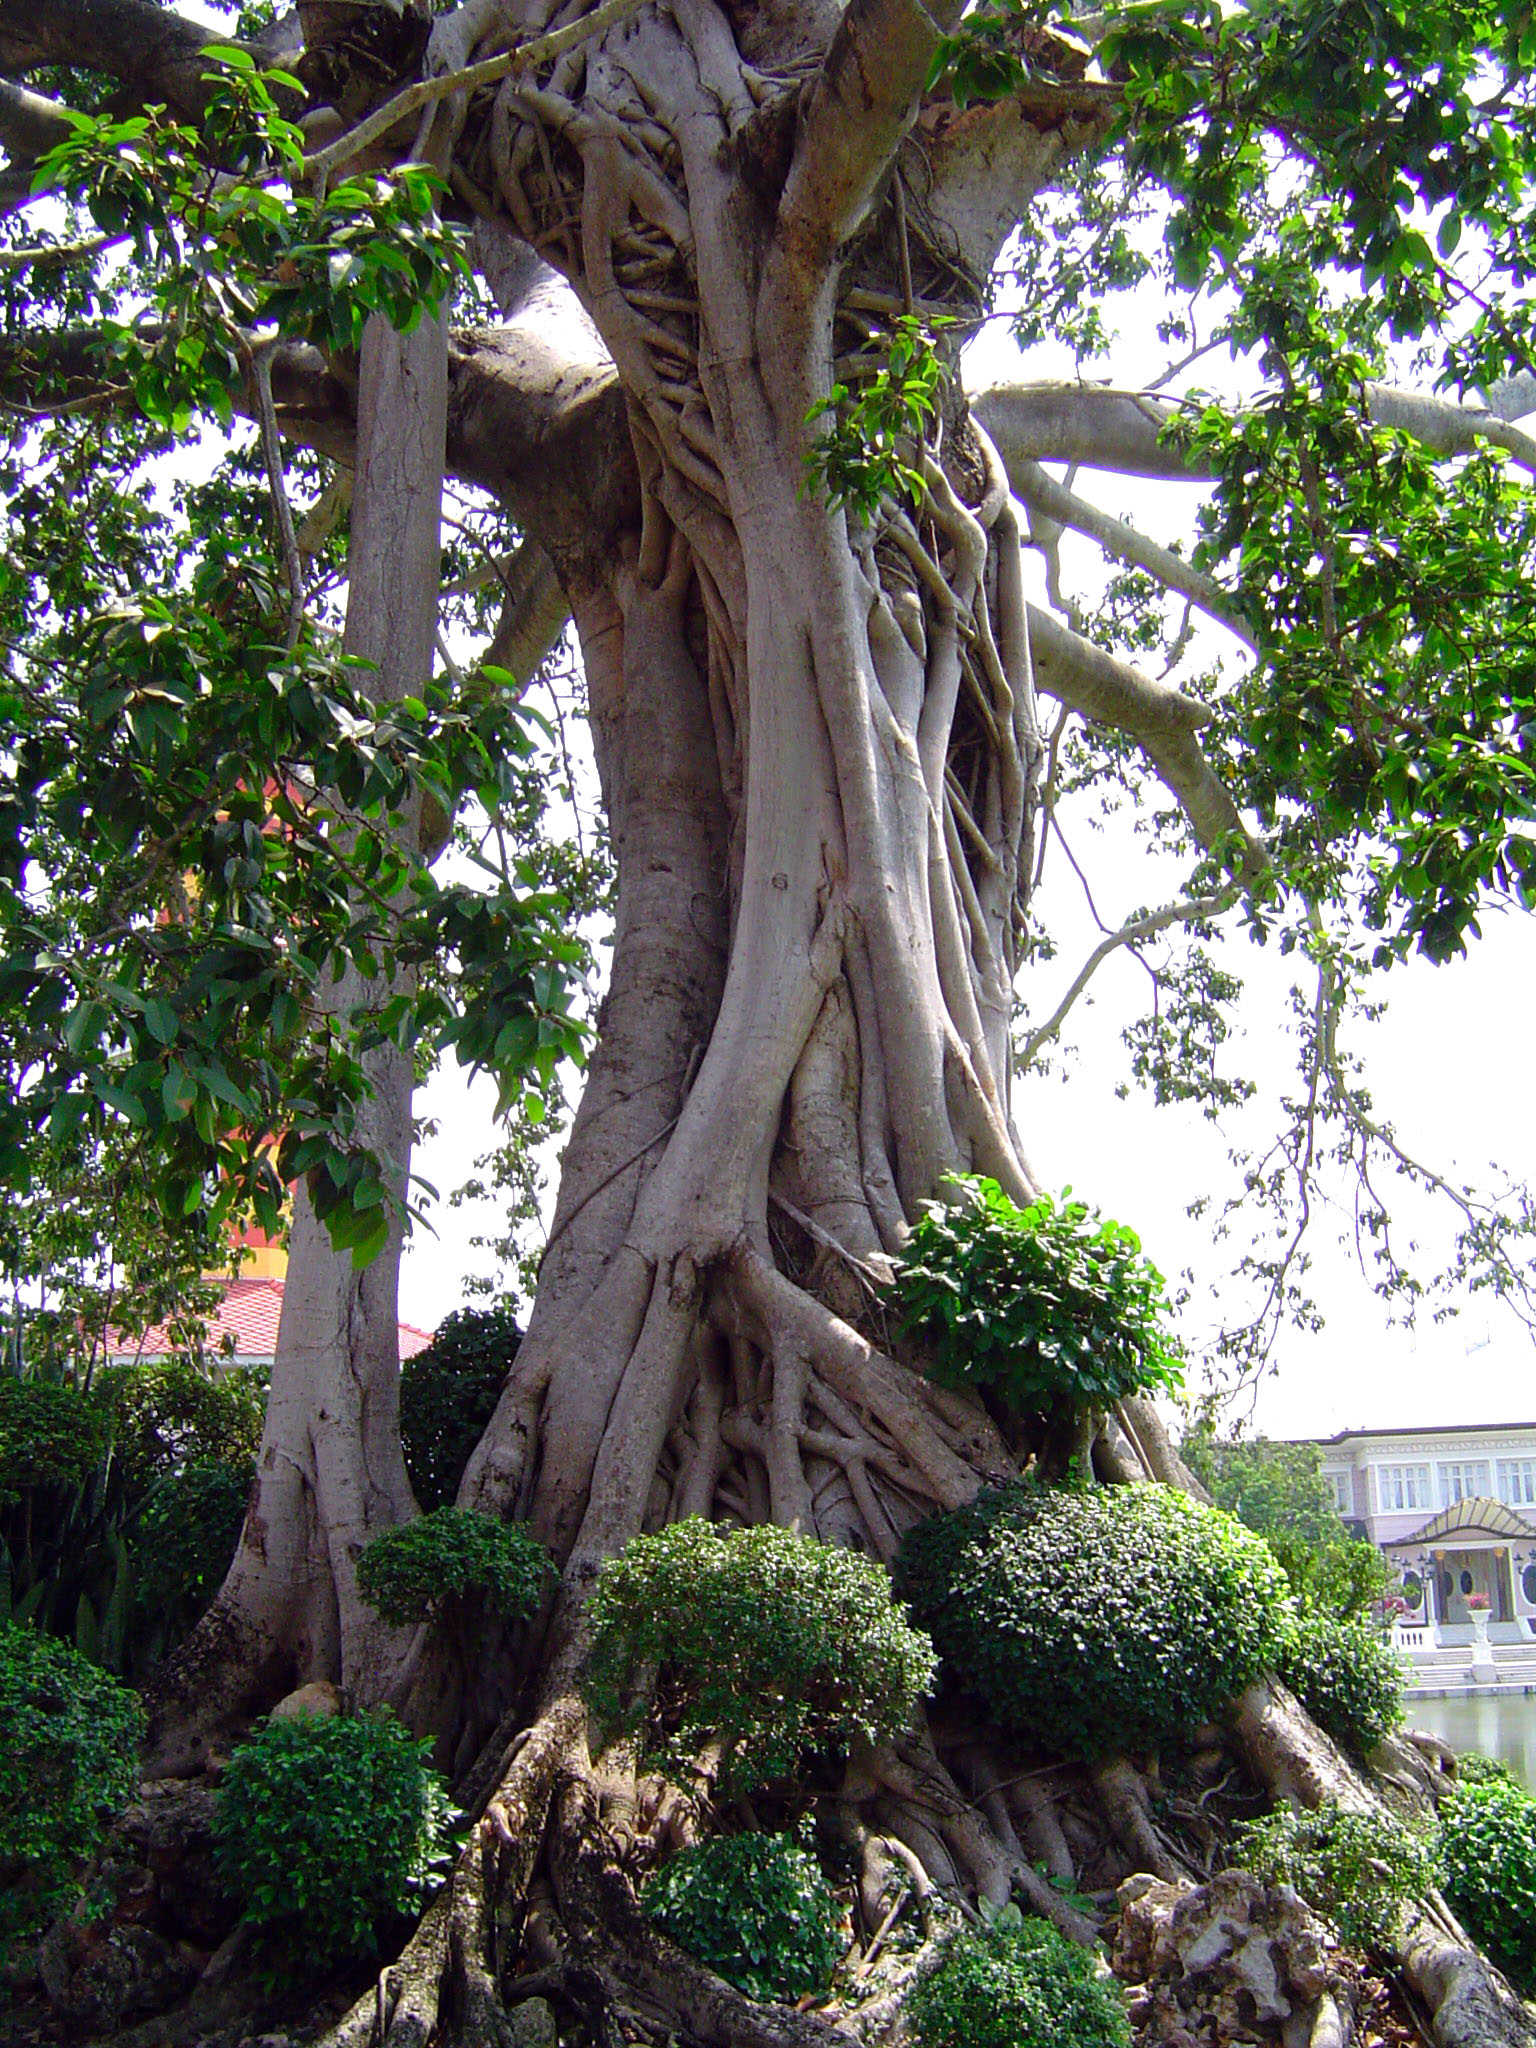
\includegraphics[width=8cm]{Ficus_in_Bang_Pa_In.jpg}\end{center}
\end{frame}
\begin{frame}
\frametitle{Dělení dvouděložných}
	\framesubtitle{Konopovité}mají žláznaté chlupy

Příklad: konopí seté

\begin{center}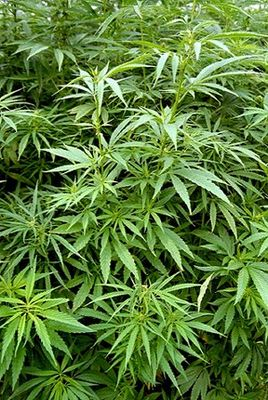
\includegraphics[width=8cm]{268px-Cannabis_sativa.jpg}\end{center}
\end{frame}
\begin{frame}
\frametitle{Dělení dvouděložných}
	\framesubtitle{Kopřivovité}mají žahavé chlupy

Příklad: kopřiva dvoudomá

\begin{center}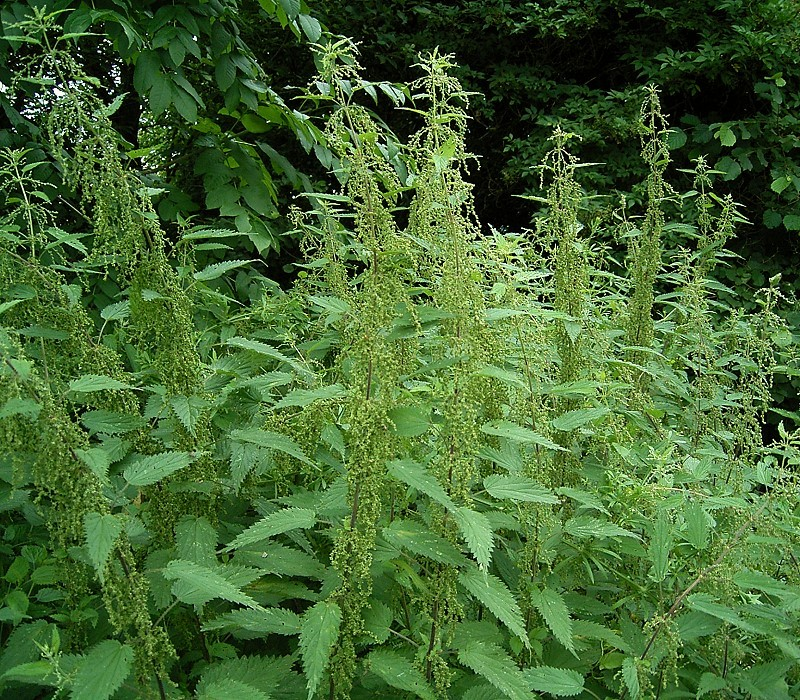
\includegraphics[width=8cm]{Urtica_dioica06_ies.jpg}\end{center}
\end{frame}
\begin{frame}
\frametitle{Dělení dvouděložných}
	\framesubtitle{Vavřínovité}(aromatické)např. avokádo

\begin{center}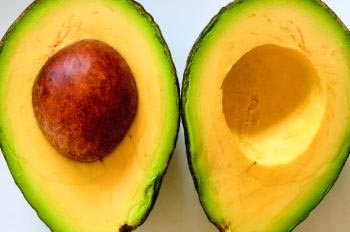
\includegraphics[width=8cm]{Avokado.jpg}\end{center}
\end{frame}
\begin{frame}
\frametitle{Dělení dvouděložných}
	\framesubtitle{Bukovité}Dřeviny

Příklad: buk lesní

\begin{center}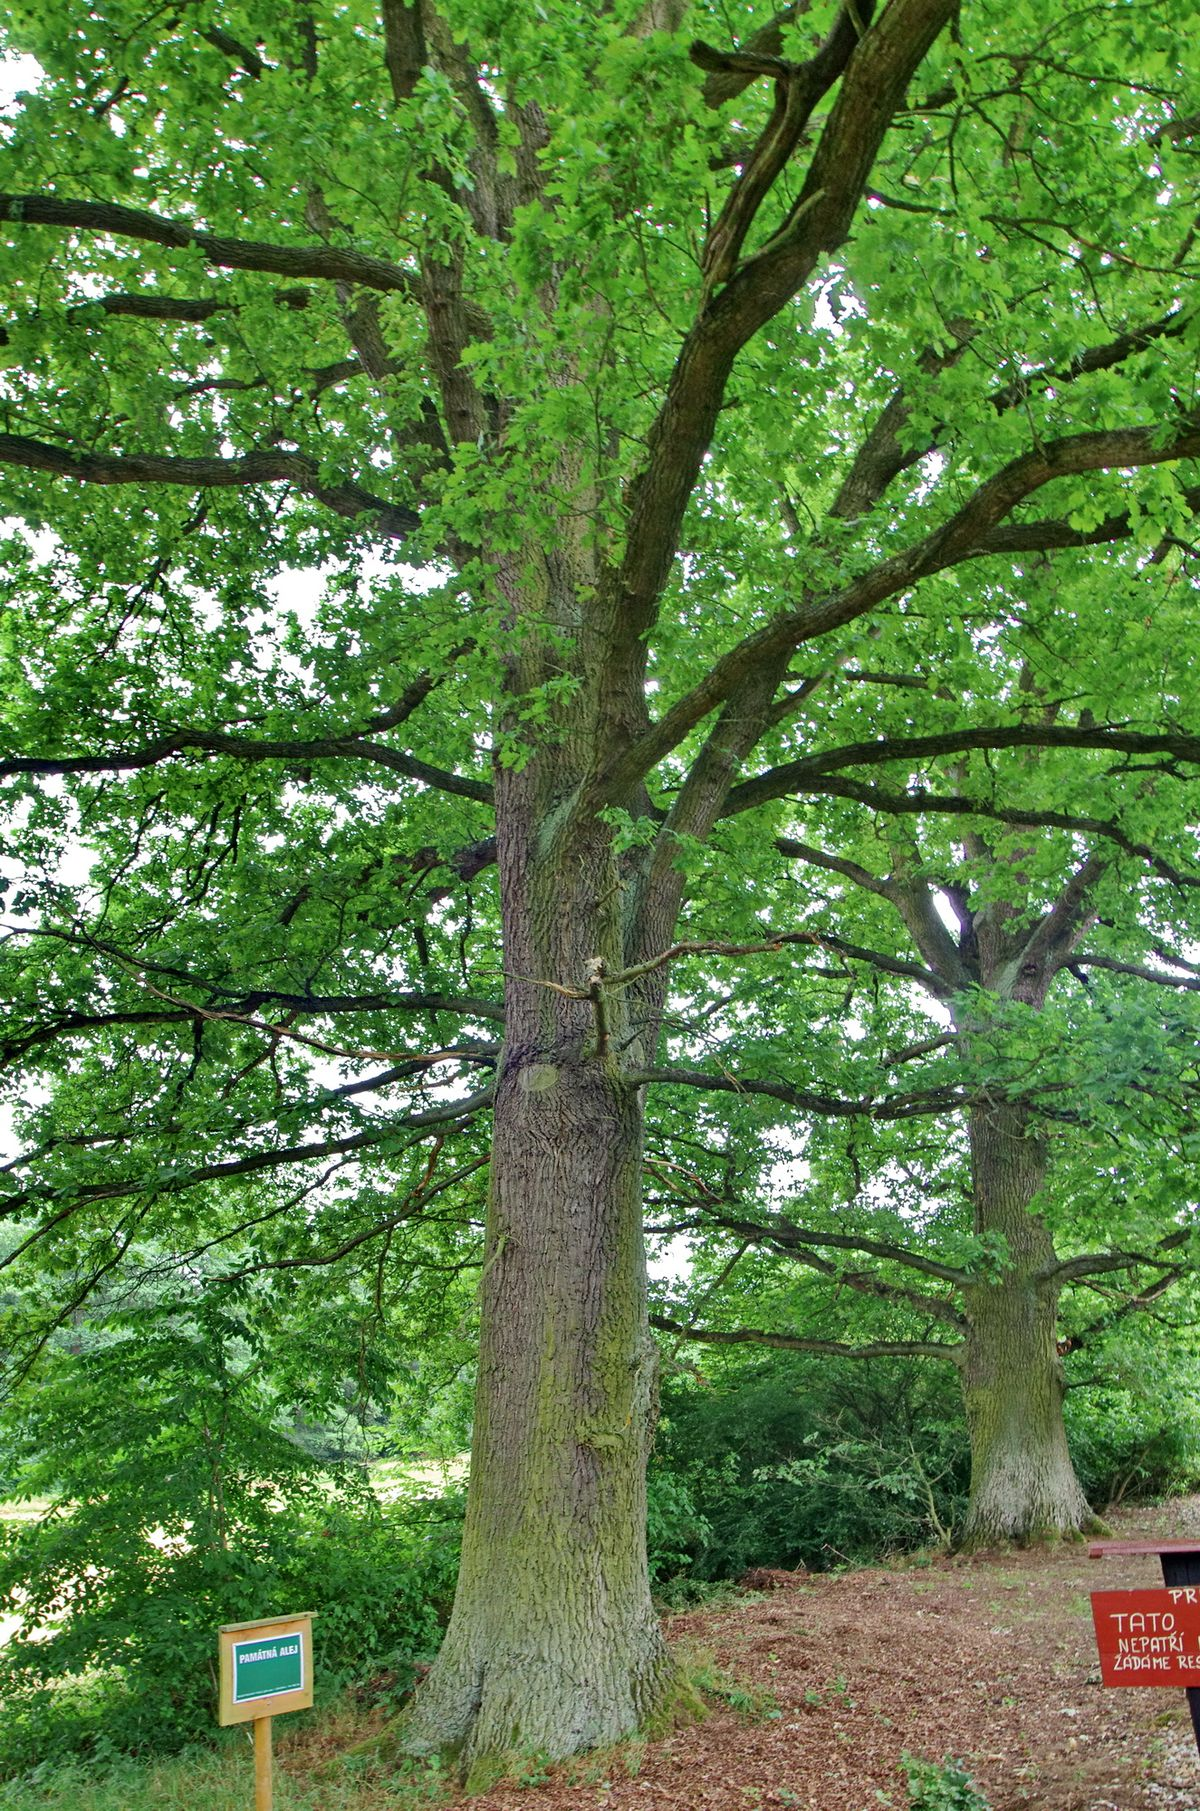
\includegraphics[width=8cm]{Buk_a_dub_v_Doubrave.jpg}\end{center}
\end{frame}
\begin{frame}
\frametitle{Dělení dvouděložných}
	\framesubtitle{Břízovité}Jednopohlavné

Příklad: bříza bělokorá

\begin{center}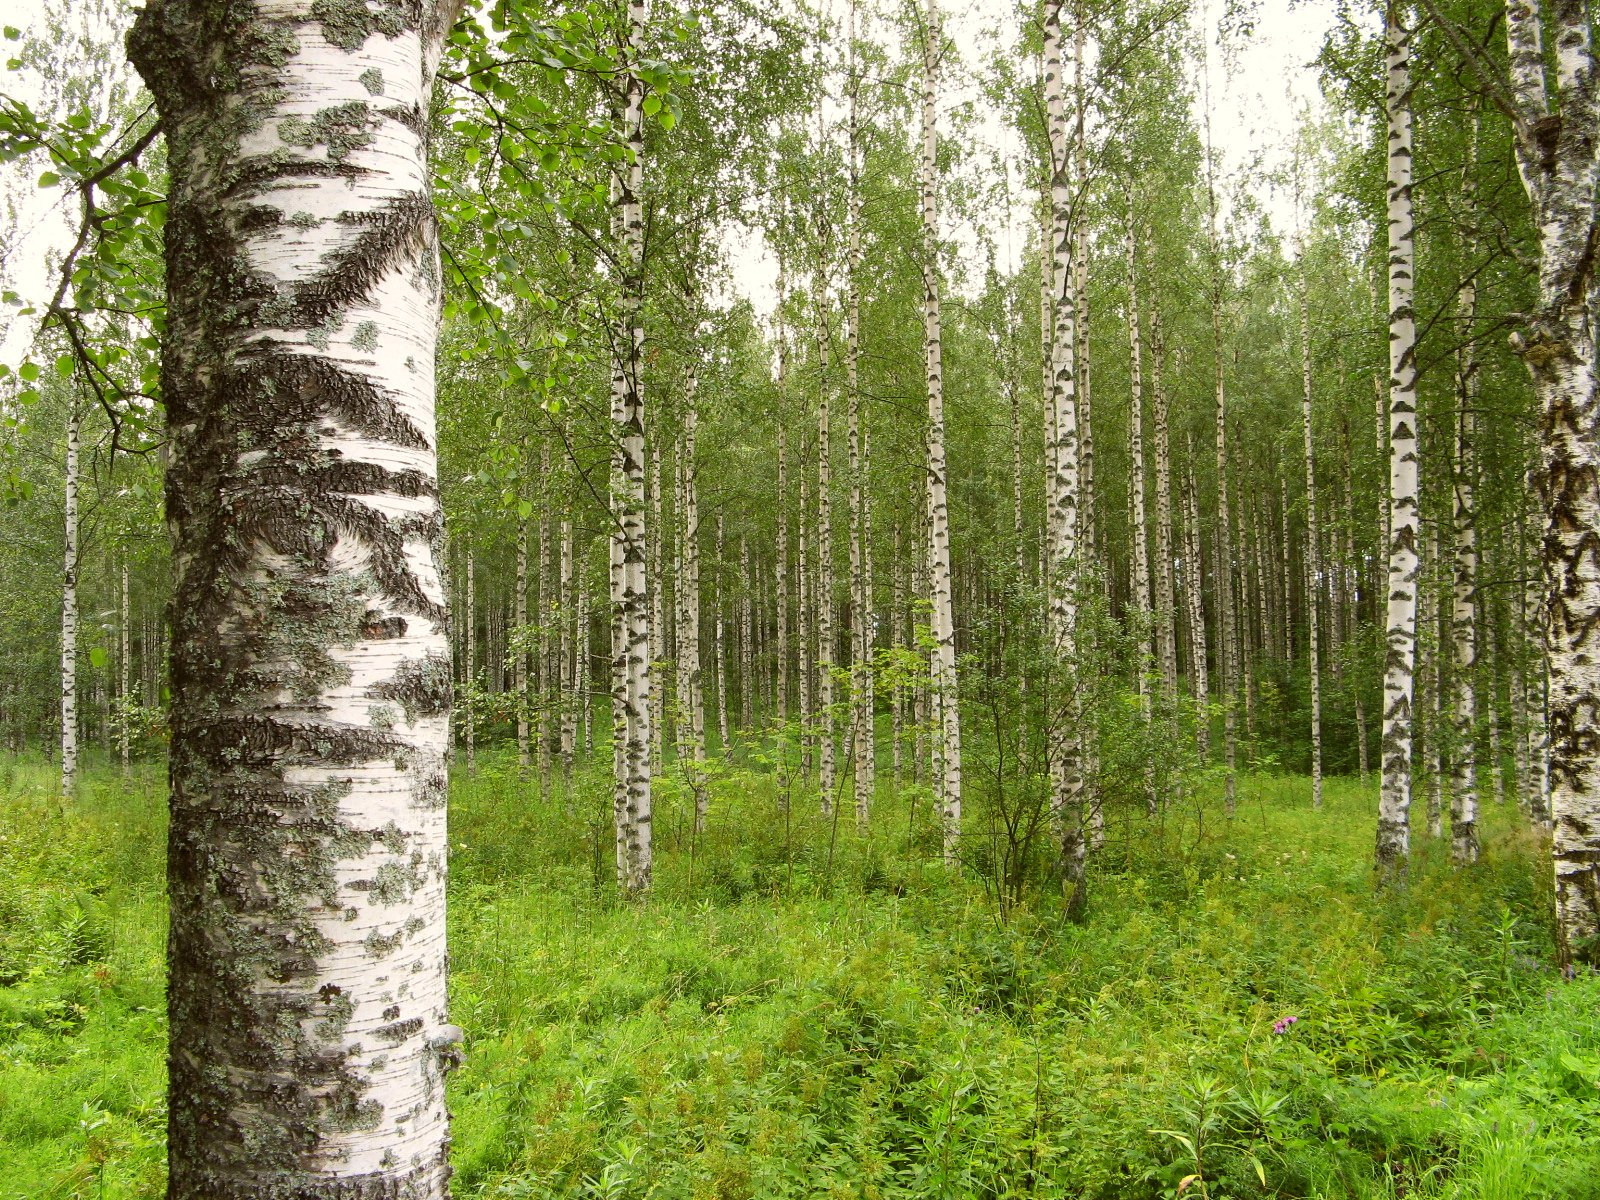
\includegraphics[width=8cm]{BirkenwaldFinnland.jpg}\end{center}
\end{frame}
\begin{frame}
\frametitle{Dělení dvouděložných}
	\framesubtitle{Merlíkovité}vrcholičnatá květenství

Příklad: řepa

\begin{center}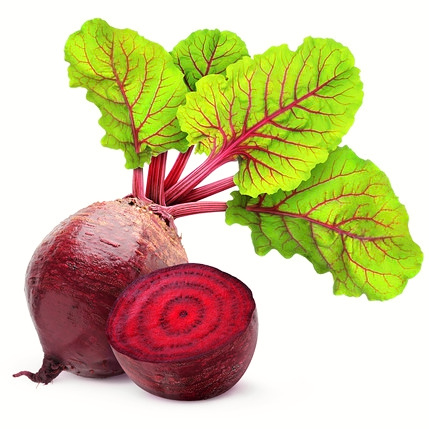
\includegraphics[width=8cm]{ico-cervena-repa.jpg}\end{center}
\end{frame}
\begin{frame}
\frametitle{Dělení dvouděložných}
	\framesubtitle{Tykvovité}poléhavé nebo popínavé, plod je bobule

Příklad: dýně

\begin{center}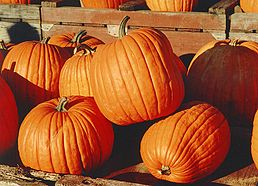
\includegraphics[width=8cm]{258px-Pumpkins.jpg}\end{center}
\end{frame}
\begin{frame}
\frametitle{Dělení dvouděložných}
	\framesubtitle{Brukvovité}mají hroznovitá květenství

Příklad: řepka olejka

\begin{center}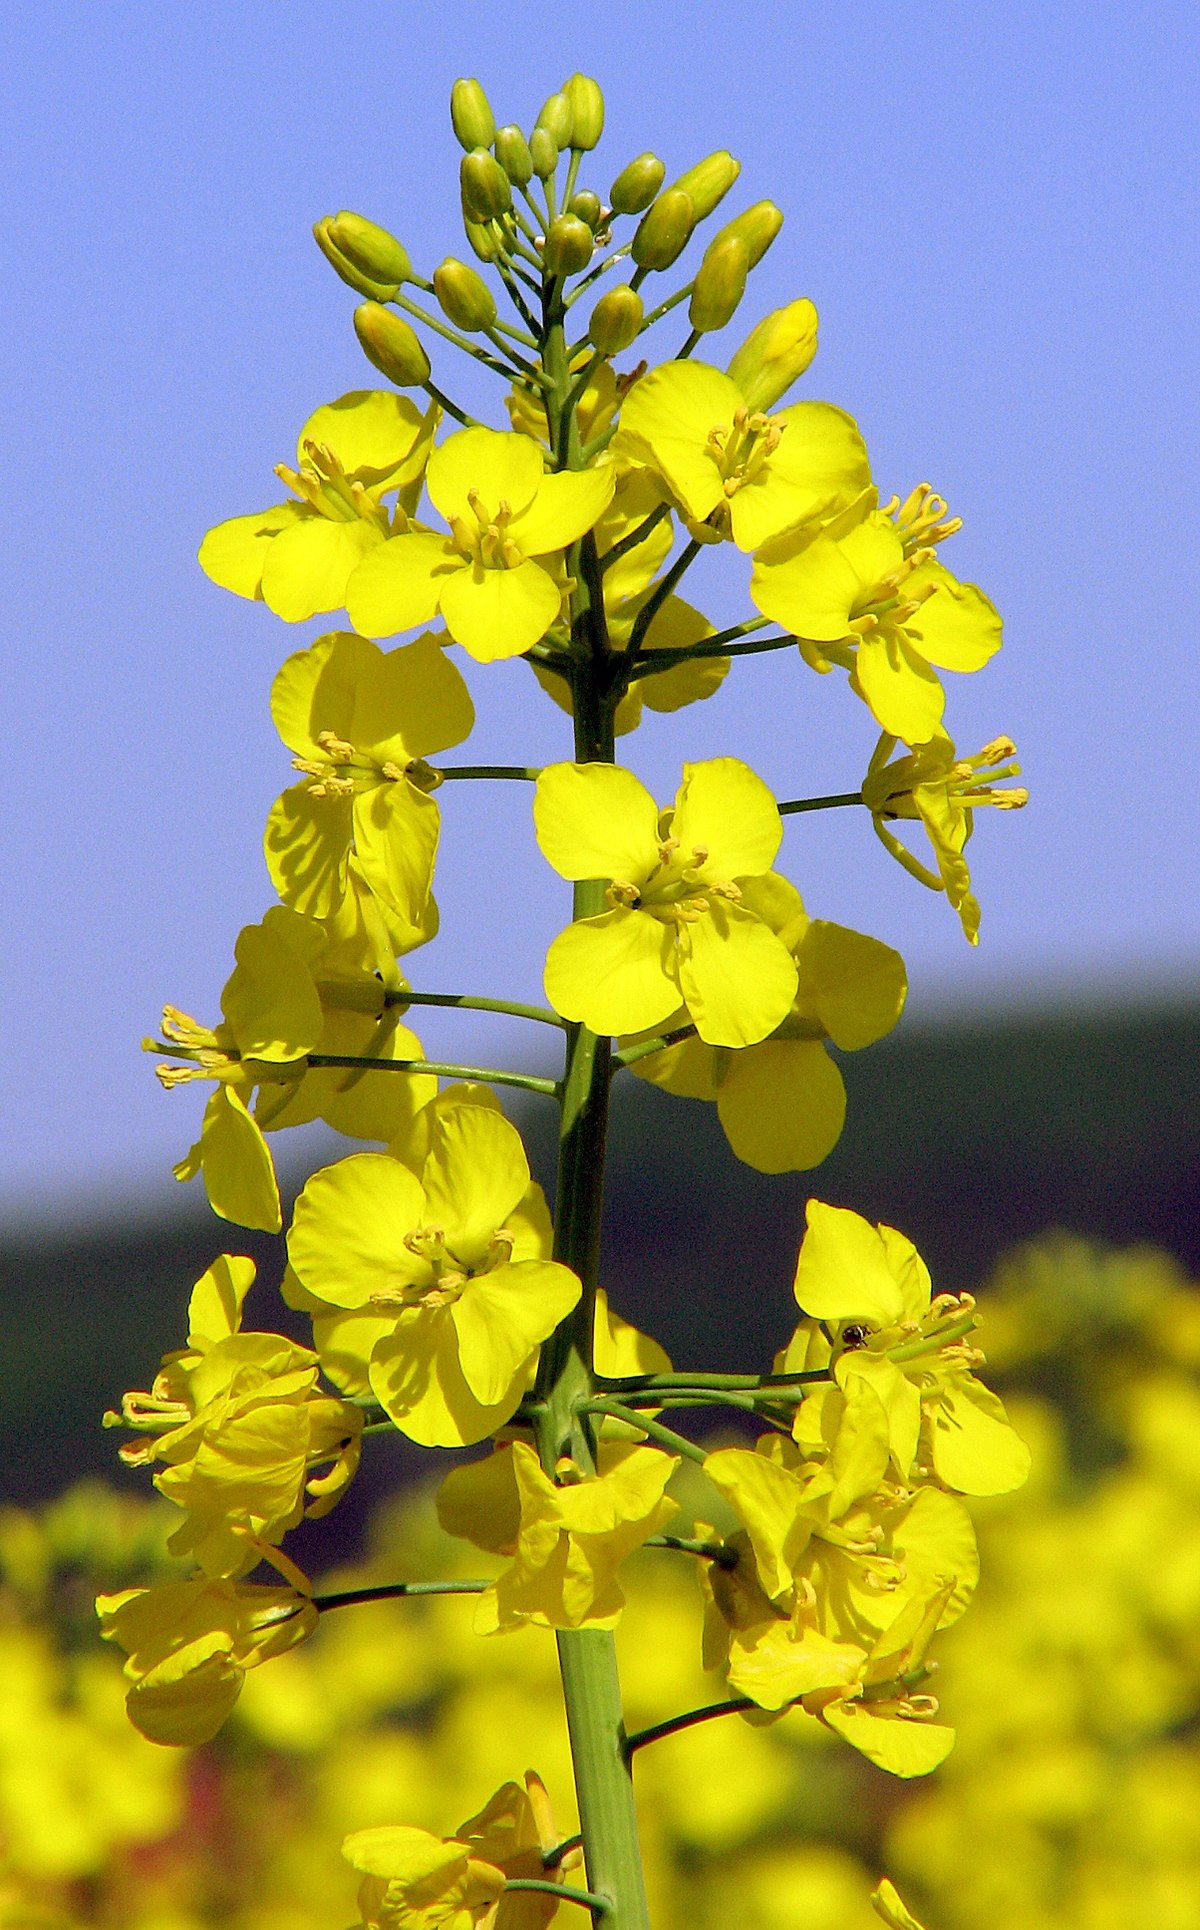
\includegraphics[width=8cm]{1200px-Brassica_napus_2.jpg}\end{center}
\end{frame}
\begin{frame}
\frametitle{Dělení dvouděložných}
	\framesubtitle{Vrbovité}bezobalné rostliny

Příklad: topol, vrba

\begin{center}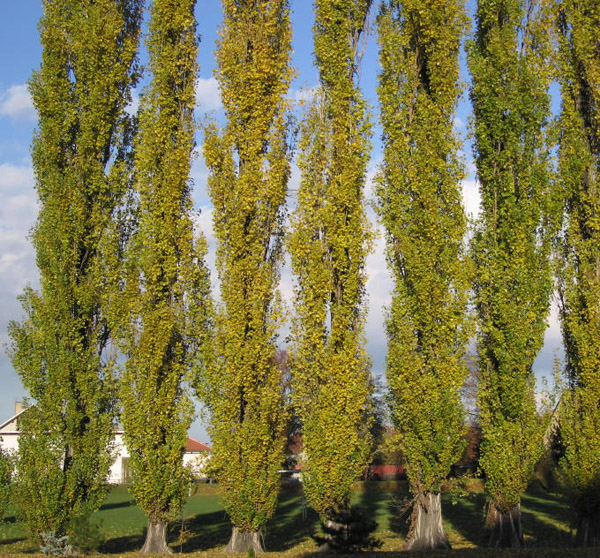
\includegraphics[width=8cm]{topol.jpg}\end{center}
\end{frame}
\begin{frame}
\frametitle{Dělení dvouděložných}
	\framesubtitle{Lomikamenovité}vysoko postavené keře

Příklad: např. rybíz

\begin{center}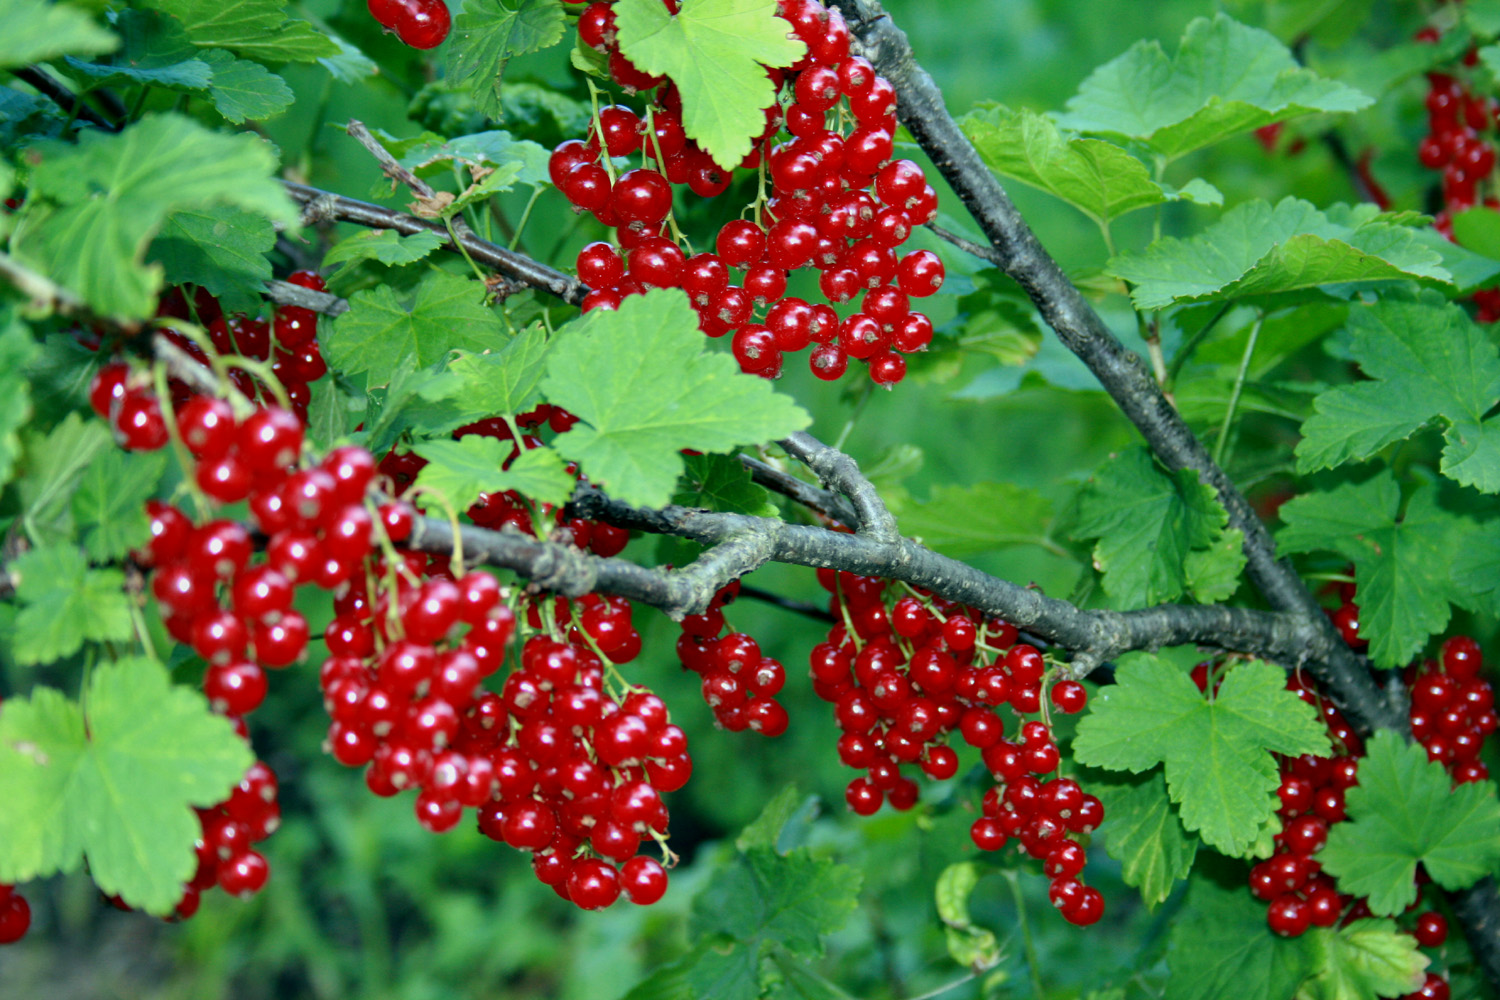
\includegraphics[width=8cm]{Cerveny_rybiz.jpg}\end{center}
\end{frame}
\begin{frame}
\frametitle{Dělení dvouděložných}
	\framesubtitle{Tlusticovité}v suchých oblastech

Příklad: rozchodník bílý

\begin{center}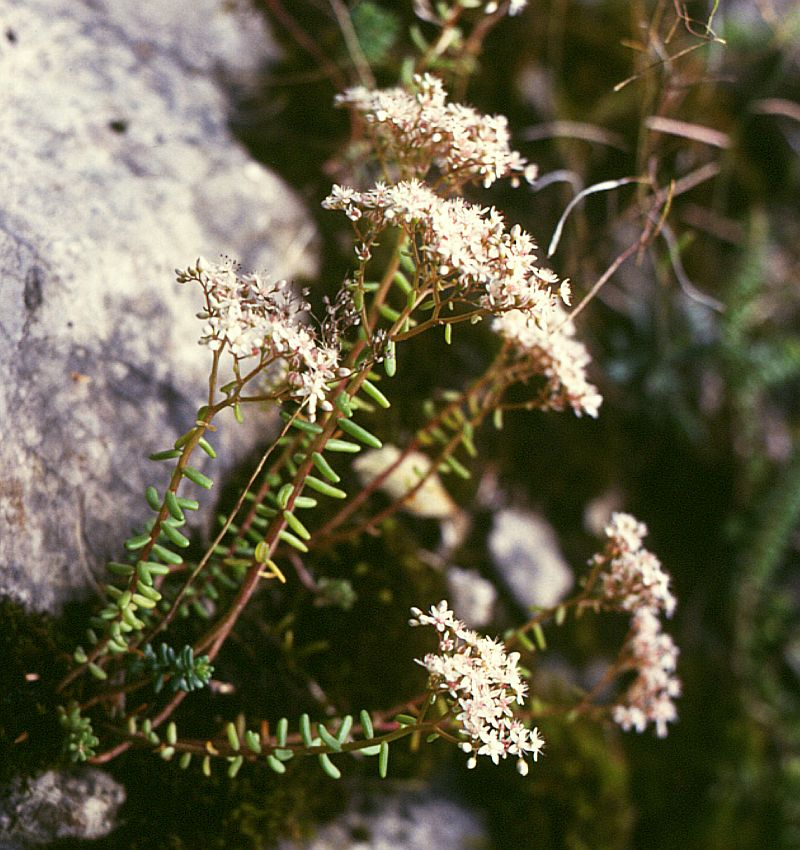
\includegraphics[width=8cm]{Sedum_album.jpg}\end{center}
\end{frame}
\begin{frame}
\frametitle{Dělení dvouděložných}
	\framesubtitle{Bobovité}mají hlízkové bakterie

Příklad: fazole, hrášek

\begin{center}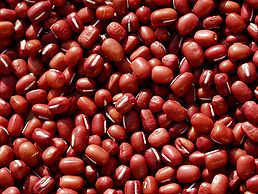
\includegraphics[width=8cm]{258px-W_azuki2111.jpg}\end{center}
\end{frame}
\begin{frame}
\frametitle{Dělení dvouděložných}
	\framesubtitle{Miříkovité}mají drobné bílé květy

Příklad: petržel

\begin{center}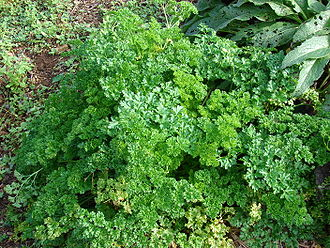
\includegraphics[width=8cm]{330px-Starr_070112-3391_Petroselinum_crispum.jpg}\end{center}
\end{frame}



\begin{frame}
\frametitle{Dělení dvouděložných}
	\framesubtitle{Brutnákovité}mají tvrdé trichomy

Příklad: pomněnka

\begin{center}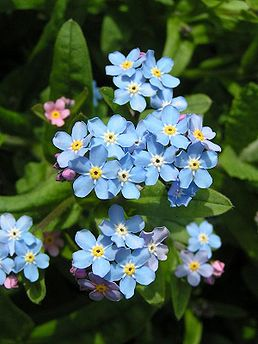
\includegraphics[width=8cm]{258px-Forget-me-not_close_600.jpg}\end{center}
\end{frame}


\begin{frame}
\frametitle{Dělení dvouděložných}
	\framesubtitle{Lilkovité}kulturní plodiny

Příklad: mandragora

\begin{center}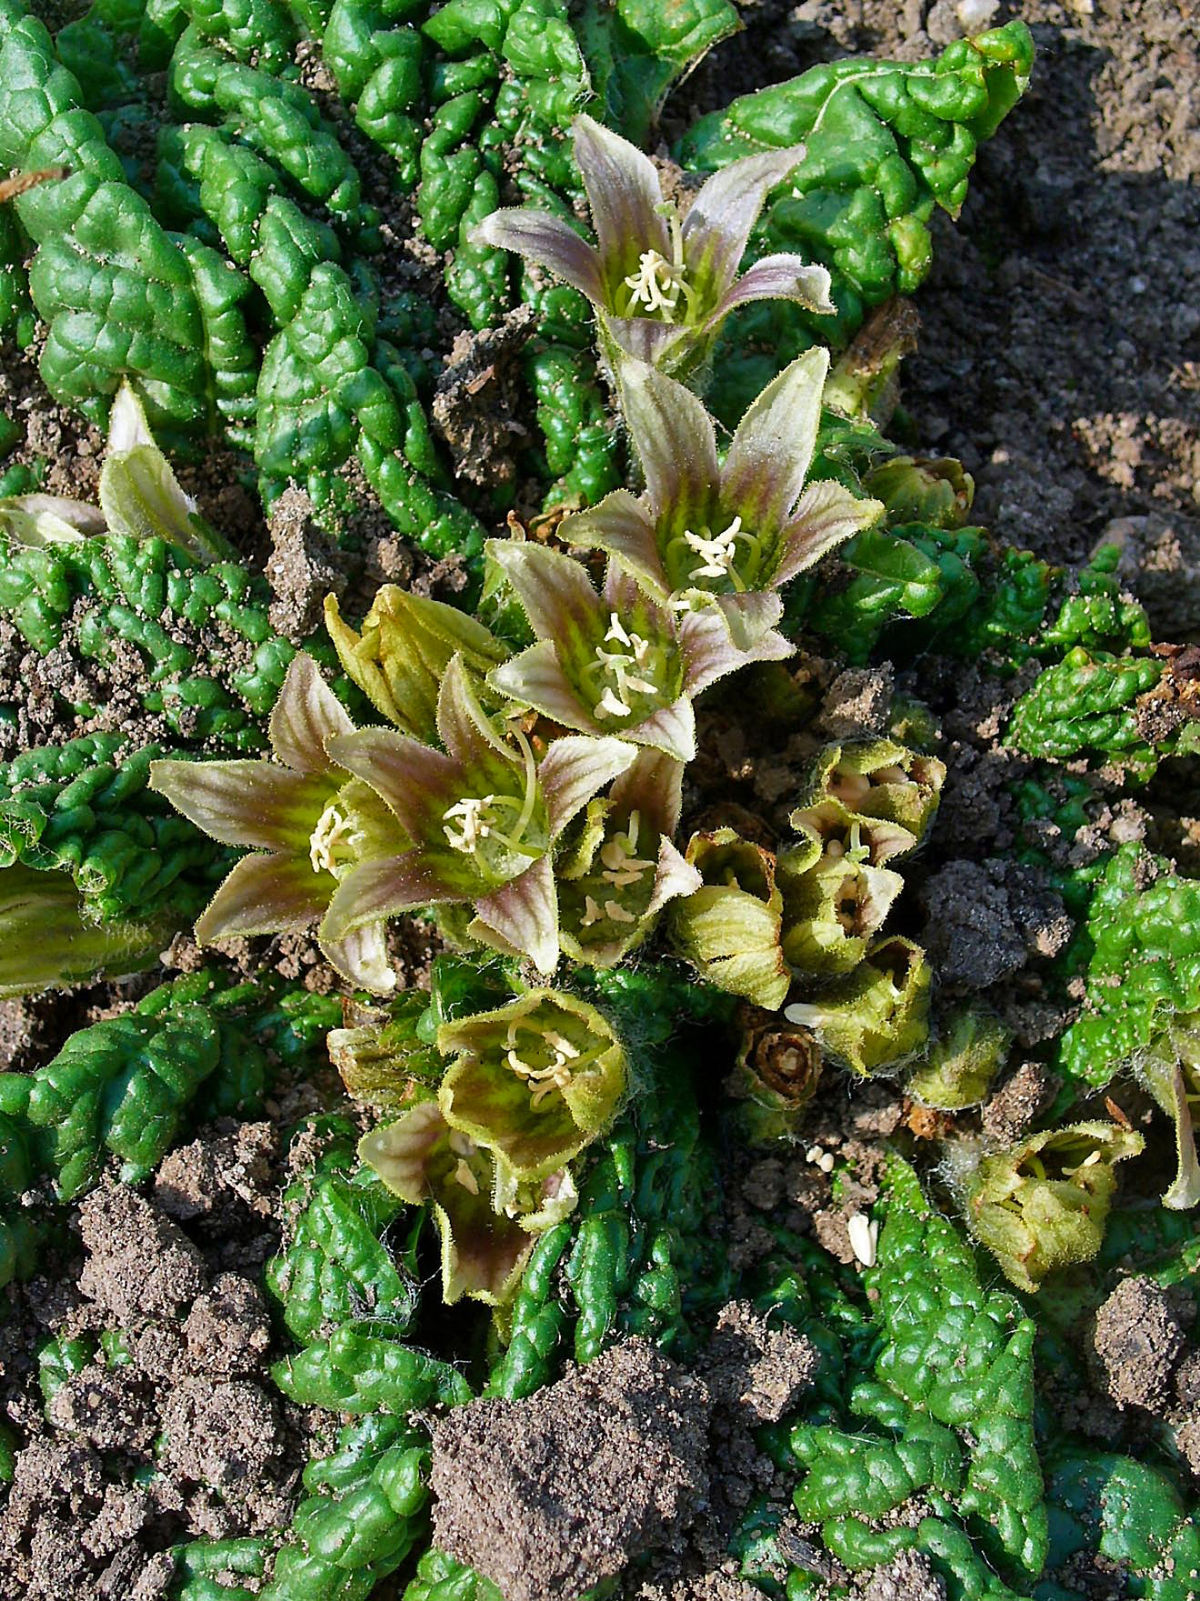
\includegraphics[width=8cm]{Mandragora_officinarum_002.jpg}\end{center}
\end{frame}

\begin{frame}
\frametitle{Dělení dvouděložných}
	\framesubtitle{Krtičníkovité}autotrofní, hemiparazité, holoparazité, mixotrofní

Příklad: rozrazil rezekvítek

\begin{center}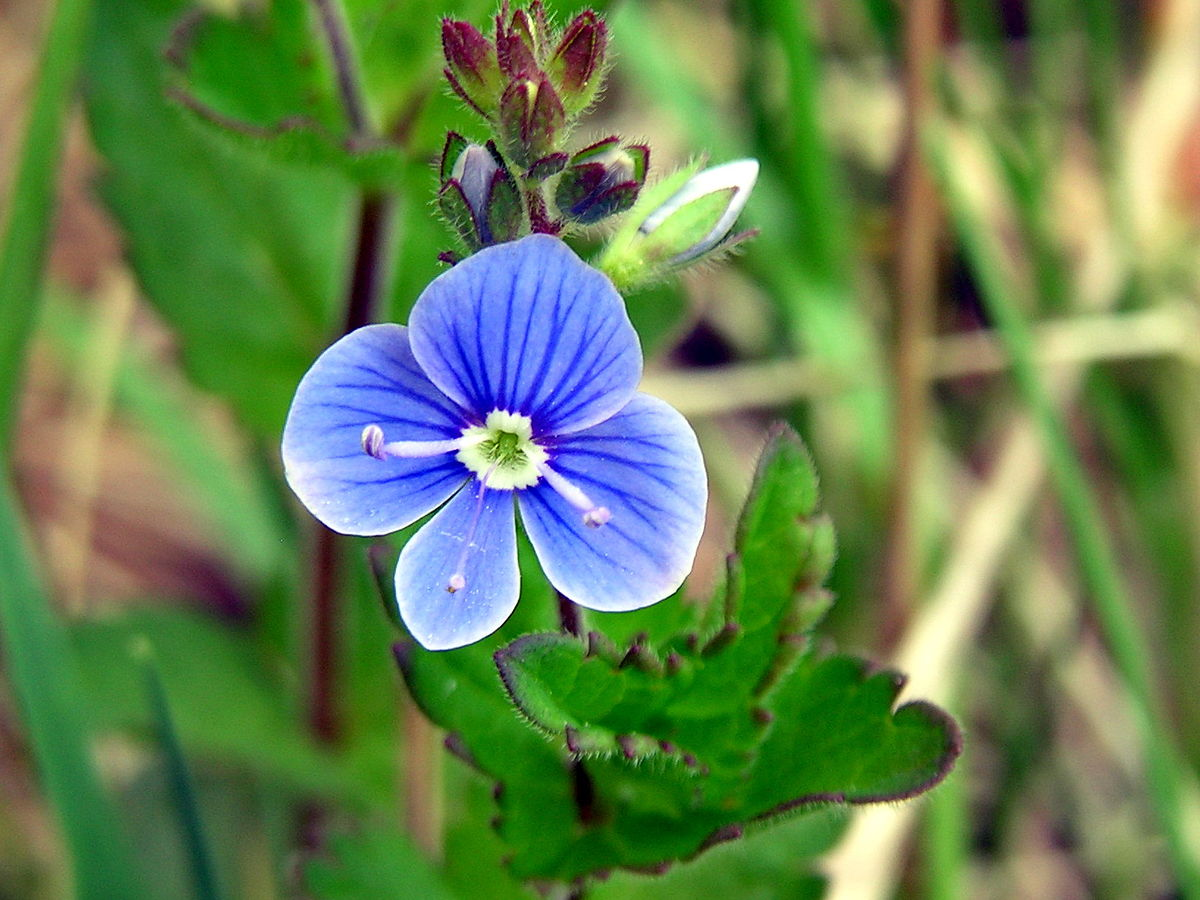
\includegraphics[width=8cm]{1200px-Veronica_chamaedrys_ziedas.jpg}\end{center}
\end{frame}
\begin{frame}
\frametitle{Dělení dvouděložných}
	\framesubtitle{Hvozdíkovité}vrcholičnatá květenství

Příklad: koukol polní

\begin{center}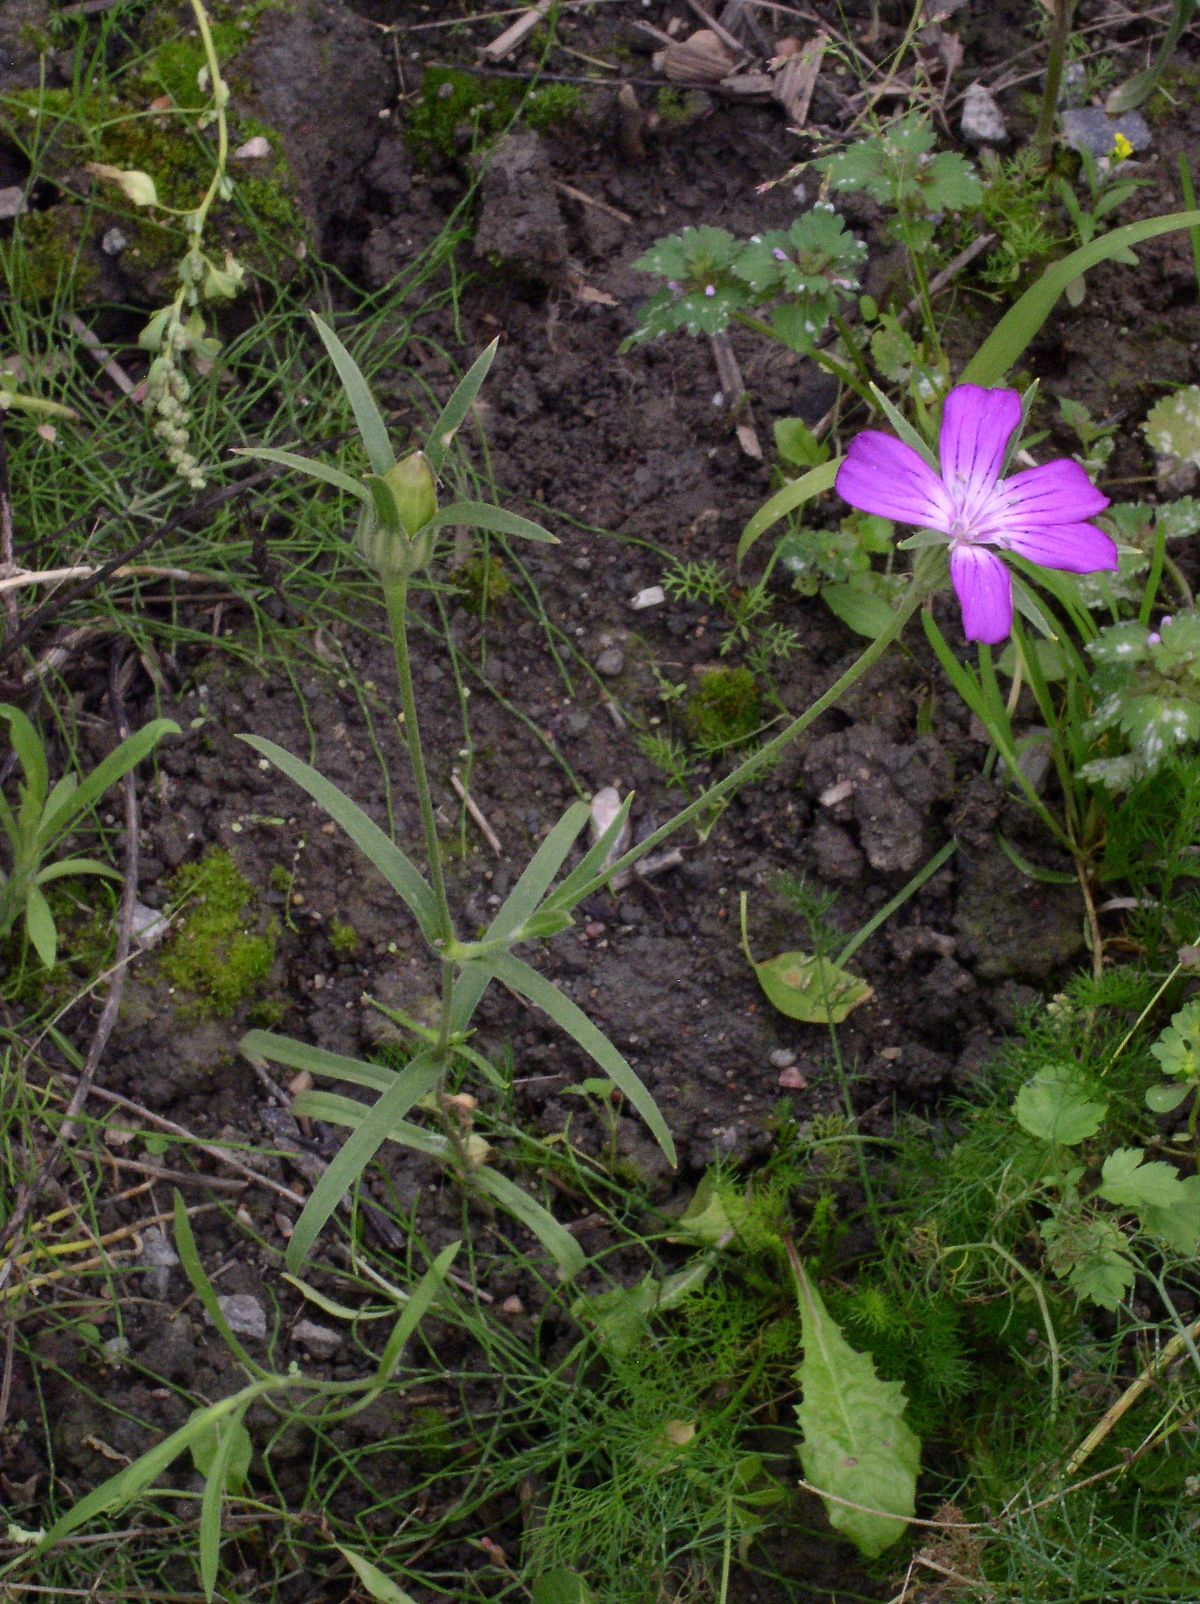
\includegraphics[width=8cm]{1200px-Agrostemma_githago_habitus_1_AB.jpg}\end{center}
\end{frame}
\begin{frame}
\frametitle{Dělení dvouděložných}
	\framesubtitle{Hluchavkovité}čtvercový stonek

Příklad: hluchavka bílá

\begin{center}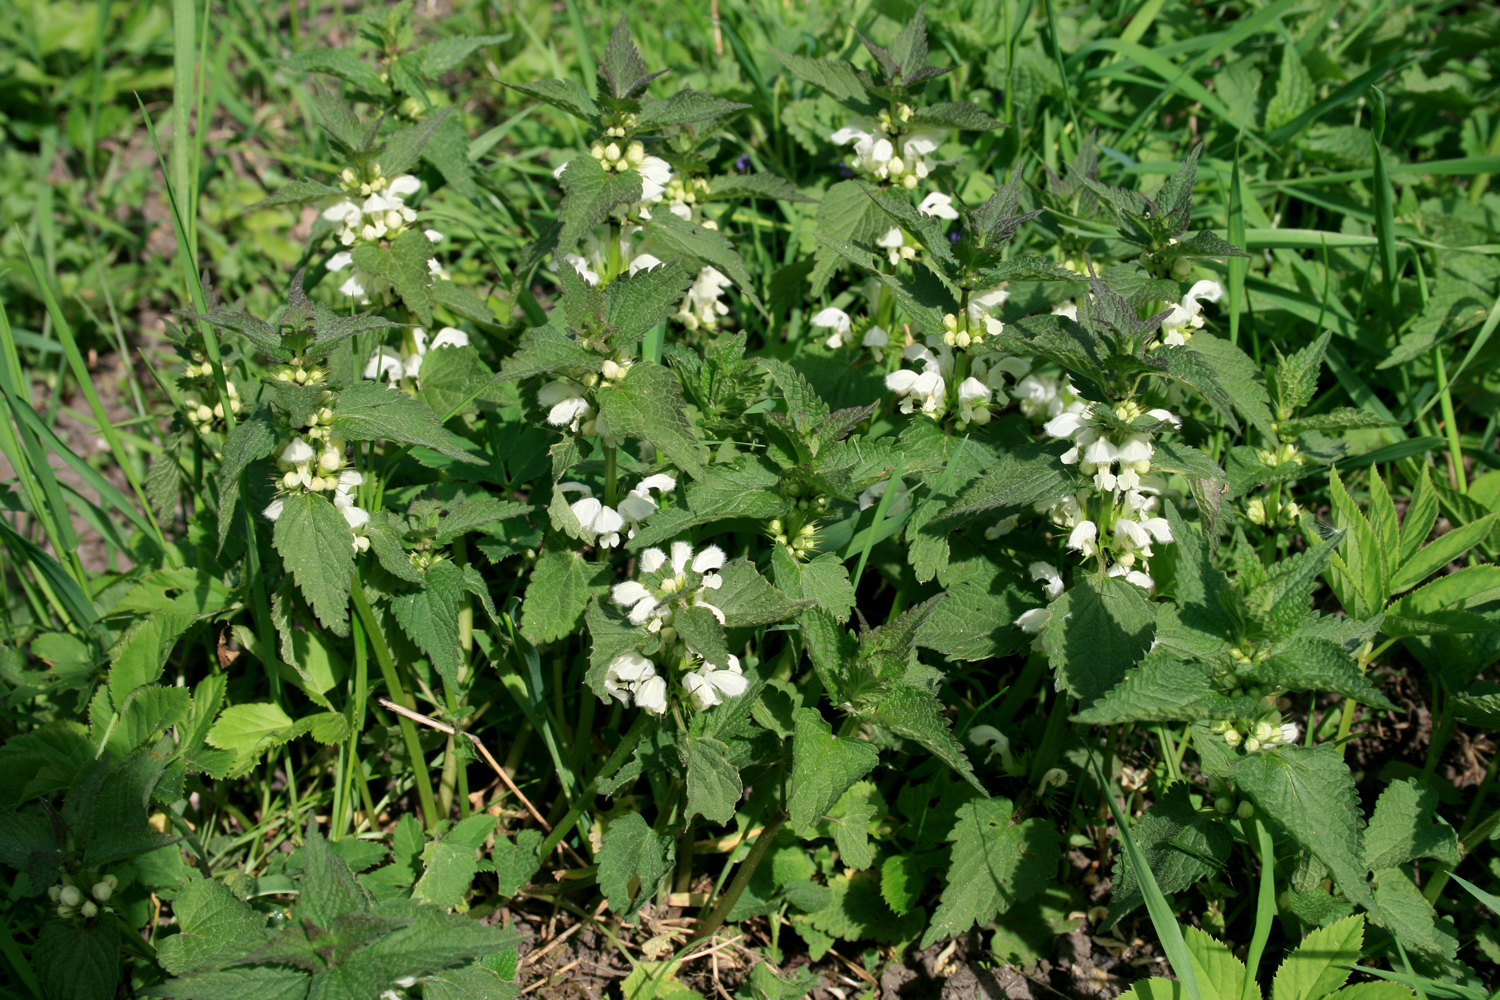
\includegraphics[width=8cm]{Hluchavka.jpg}\end{center}
\end{frame}
\begin{frame}
\frametitle{Dělení dvouděložných}
	\framesubtitle{Hvězdnicovité}nejpočetnější, nejrozmanitější

Příklad: bodláky

\begin{center}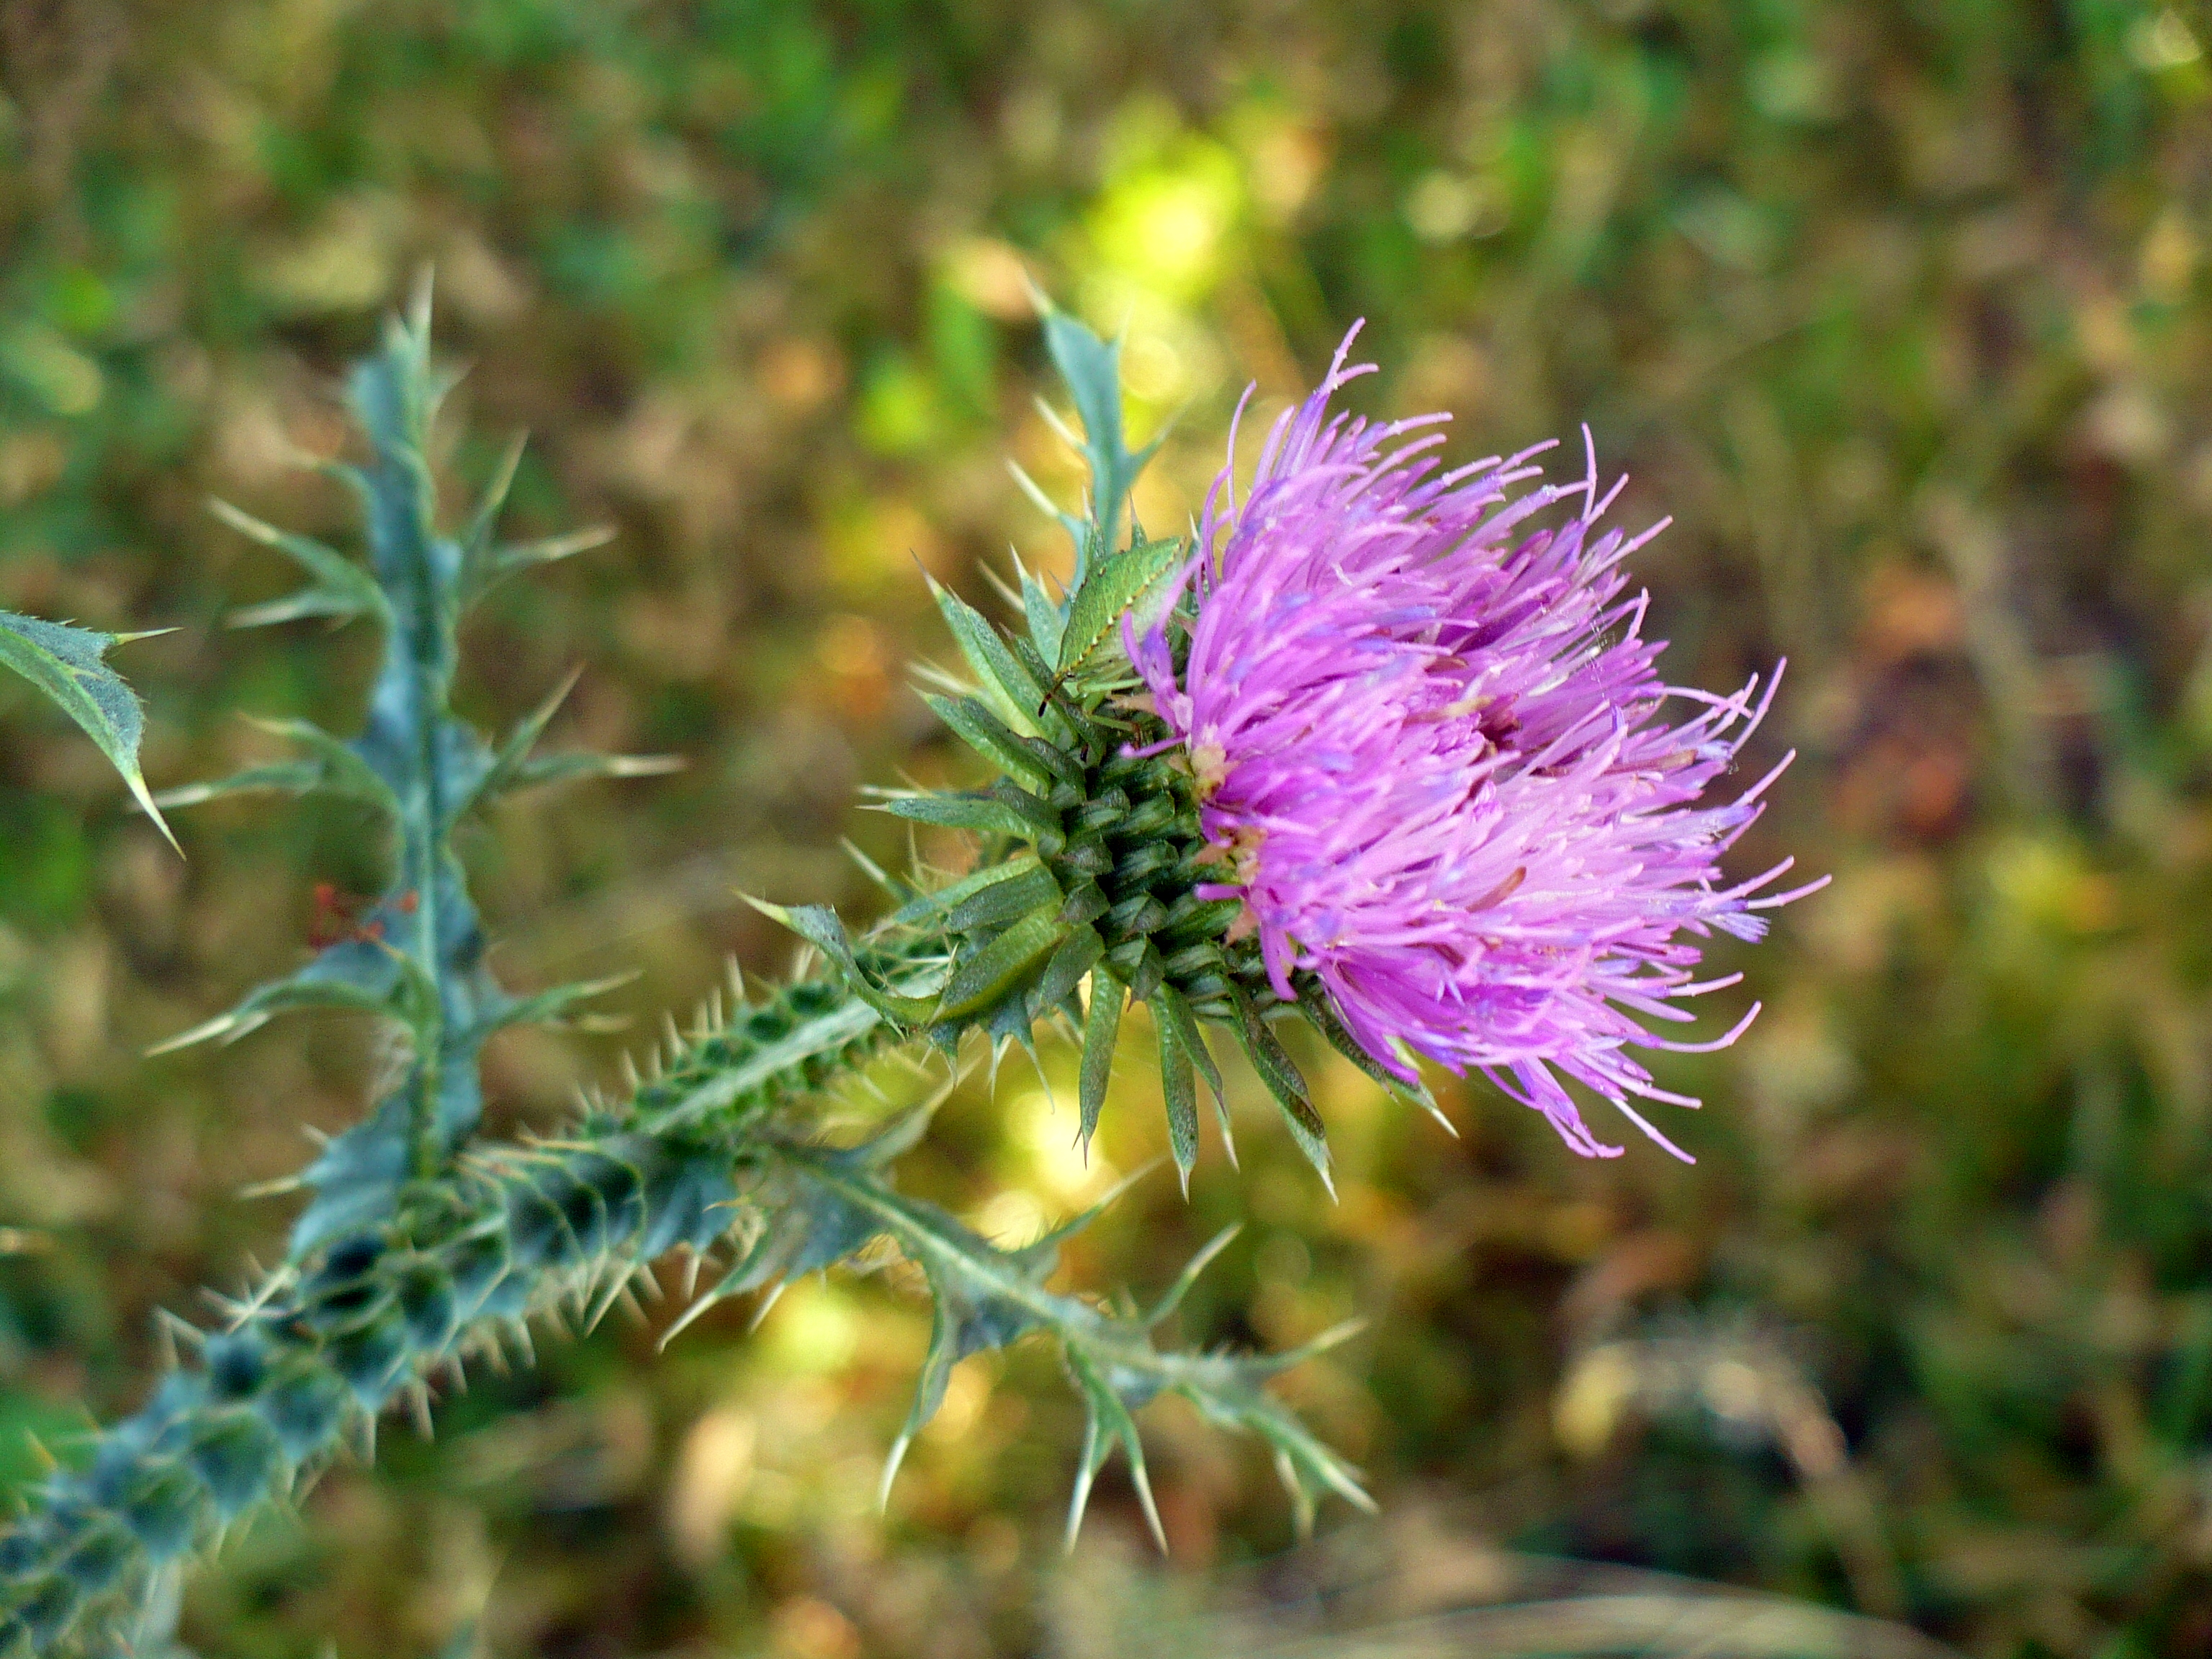
\includegraphics[width=8cm]{Carduus_acanthoides_syp_4.jpg}\end{center}
\end{frame}
\begin{frame}
\frametitle{Dělení dvouděložných}
	\framesubtitle{Růžovité}byliny i dřeviny

Příklad: jahodník obecný, třešeň ptačí, jabloň domácí

\begin{center}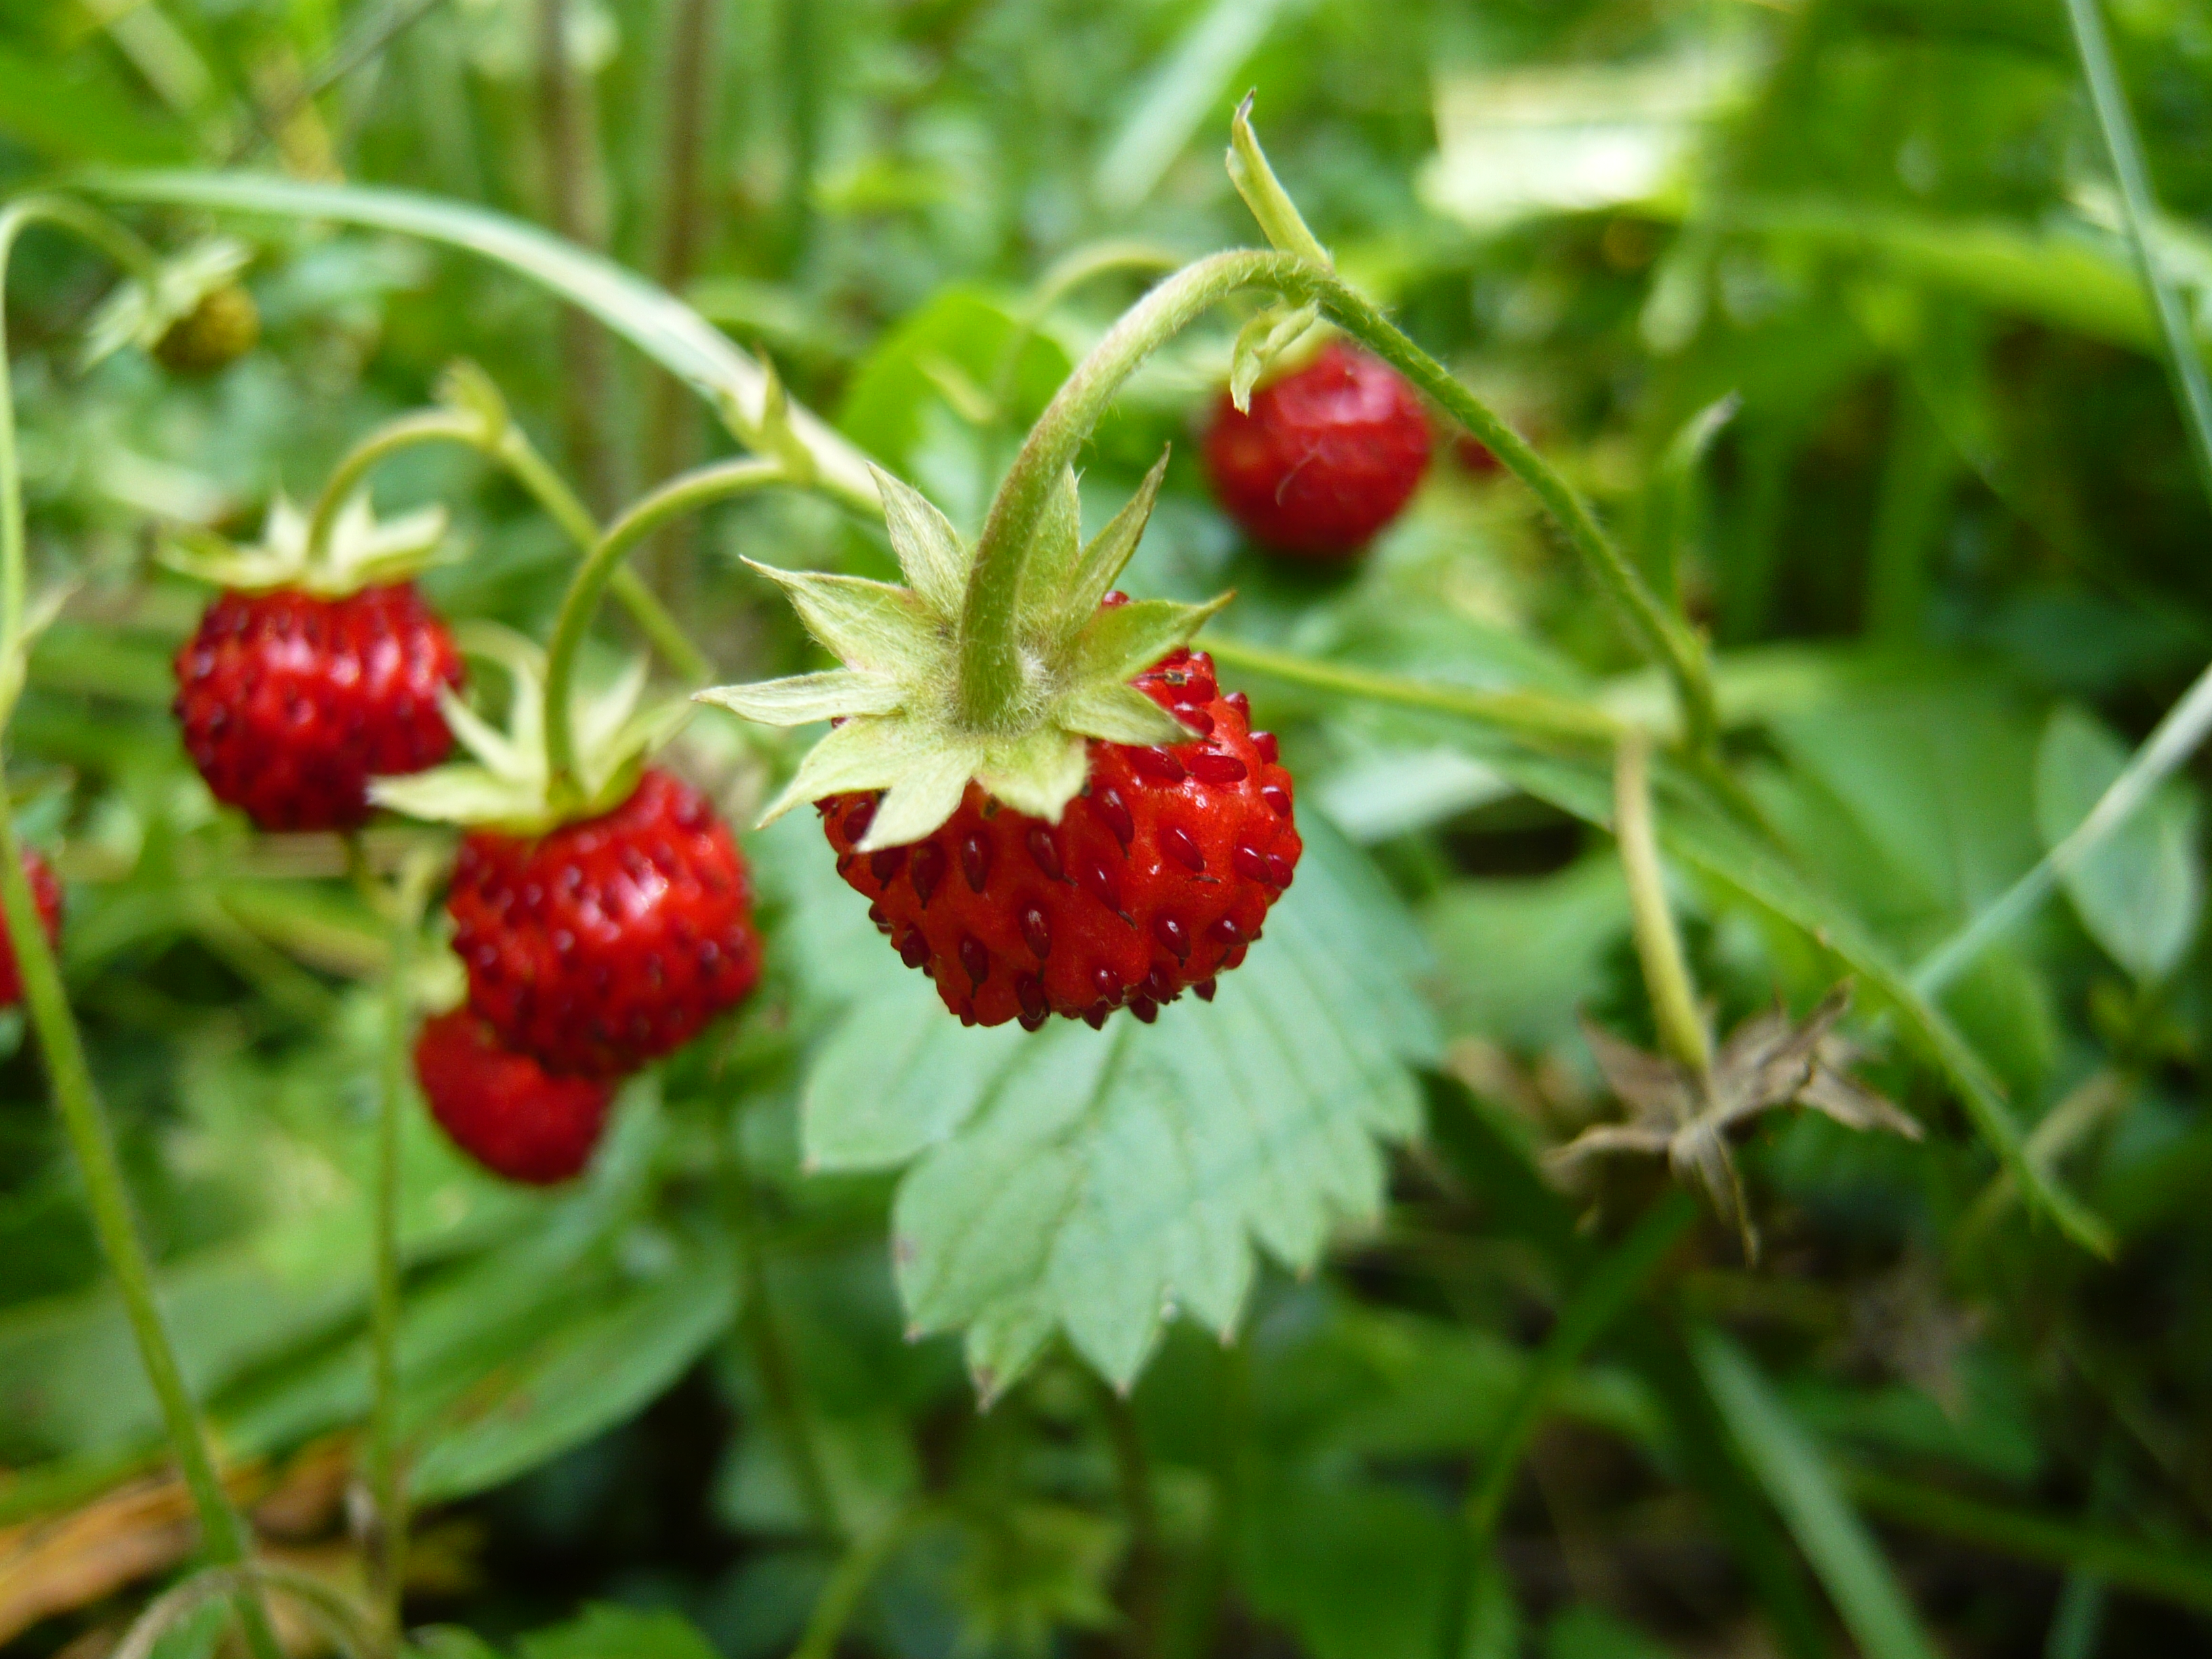
\includegraphics[width=8cm]{Fraise_des_bois.jpg}\end{center}
\end{frame}

\begin{frame}
\frametitle{Zdroje}

http://www.szes-la.cz/

http://trpitele.blog.cz/

https://cs.wikipedia.org/

http://www.biomach.cz/





\end{frame}

\end{document}